% Source package using the supplied ICLR 2027 style; generated/ and figures/ are included.
% The current method is called NBPO throughout; earlier fixed-reference results are labeled as a precursor variant.
\documentclass{article}
\usepackage{iclr2027_conference,times}
\usepackage[hidelinks,hypertexnames=false]{hyperref}
\usepackage{url}
\usepackage{graphicx}
\usepackage{amsmath}
\usepackage{amssymb}
\usepackage{amsthm}
\usepackage{booktabs}
\usepackage{algorithm}
\usepackage{algorithmic}
\usepackage{float}
\usepackage{microtype}
\usepackage{placeins}

\newtheorem{theorem}{Theorem}
\newtheorem{lemma}{Lemma}
\newtheorem{proposition}{Proposition}
\newtheorem{corollary}{Corollary}
\newtheorem{assumption}{Assumption}
\newtheorem{definition}{Definition}
\theoremstyle{remark}
\newtheorem{remark}{Remark}
\theoremstyle{plain}

\newcommand{\Y}{\mathcal{Y}}
\newcommand{\G}{\mathcal{G}}
\newcommand{\KL}{\mathrm{KL}}
\newcommand{\E}{\mathbb{E}}
\newcommand{\R}{\mathbb{R}}
\newcommand{\D}{\mathcal{D}}
\newcommand{\piref}{\pi_{\mathrm{ref}}}
\newcommand{\NBPO}{\textsc{NBPO}}
\newcommand{\pending}{\textemdash}
\newcommand{\meanstd}[2]{\ensuremath{#1{\scriptstyle\pm#2}}}

\title{Nash Bargaining Preference Optimization}
\author{Anonymous authors}
%\iclrfinalcopy

% Generated by export_paper_tables.py:residual_macros -- do not hand-edit.
% Source: results/iclr2027_table1_v2/controlled_v2/controlled_v2_raw.json
\newcommand{\ControlledMaxKKT}{\ensuremath{6.2\times10^{-9}}}
\newcommand{\ControlledMaxInner}{\ensuremath{5.1\times10^{-5}}}
\newcommand{\ControlledMaxIdentity}{\ensuremath{1.5\times10^{-14}}}

\begin{document}
\maketitle

\begin{abstract}
Multi-objective alignment requires both a representation of preferences and a rule for selecting a compromise. We introduce Nash Bargaining Preference Optimization (\NBPO{}), which evaluates each objective through a regularized preference game and applies Nash bargaining to improvement over a common reference policy. A constrained KL-proximal formulation handles zero surplus at the reference; a prompt-separable finite-pool solver accounts for adaptive opponents; and pairwise log-ratio regression transfers its target to an LLM without evaluating a language-model normalizer. Exact population updates admit an $O(1/T)$ last-iterate guarantee. Controlled experiments support adaptive game values as preference nontransitivity increases. In an 8B model, short-schedule regression reduces held-out target error and finite-pool forward KL, with positive teacher-defined surpluses and near-base instruction-following and mathematics point estimates. Independent evaluation and repeated policy seeds remain necessary: the current natural panel does not establish an aggregation advantage or empirical Pareto optimality.
\end{abstract}

\section{Introduction}
\label{sec:intro}
Reinforcement Learning from Human Feedback (RLHF) is a standard approach for aligning large language models (LLMs) with human judgments \citep{christiano2017deep,ouyang2022training}. Standard RLHF learns a scalar reward from pairwise comparisons. Direct Preference Optimization removes the separately trained reward model, but still assumes that comparisons are generated by an implicit scalar reward through a Bradley--Terry (BT) model \citep{rafailov2023direct,bradley1952rank}. Both approaches therefore require every response to admit one scalar score whose ordering explains all pairwise preferences.

This assumption can fail even within a single alignment objective. Human judgments can reflect several latent attributes whose relative importance changes with the prompt and the pair being compared \citep{tversky1969intransitivity,wang2024armorm}. As an illustrative example, consider three answers to a medical-advice question. Response $A$ is concise and actionable but omits an important caveat; response $B$ is comprehensive but verbose; and response $C$ is less complete but includes the critical safety warning. Annotators may prefer $A$ to $B$ for relevance, $B$ to $C$ for completeness, and $C$ to $A$ for safety and reliability. These comparisons are cyclic: $A\succ B$, $B\succ C$, and $C\succ A$. Fitting the first two comparisons with a scalar reward requires $r(A)>r(B)>r(C)$, which contradicts the third. As a result, optimizing the fitted scalar reward can favor a response that appears best under the learned ranking but is still beaten by another response according to the original pairwise judgments \citep{munos2024nash}.

Nash Learning from Human Feedback (NLHF) avoids this misspecification by treating prompt-conditioned comparisons directly as payoffs in a zero-sum preference game, and INPO, SPPO, and related methods provide scalable equilibrium-seeking updates \citep{munos2024nash,zhang2025iterative,wu2025sppo,calandriello2024online,rosset2024direct,zhou2025egpo}. Extending this view to multiple objectives introduces a second problem: after representing each objective without imposing transitivity, which compromise should one deployed policy realize? Scalar multi-objective methods expose this trade-off through weights, priorities, constraints, policy interpolation, or preference conditioning \citep{zhou2024beyond,rame2023rewarded,zhong2024panacea,chakraborty2024maxmin,son2026rmod,agnihotri2026mopo}. Recent game-theoretic methods preserve general pairwise feedback but combine objectives through Blackwell target sets or a worst-objective criterion \citep{blackwell1956analog,bhatia2020multicriteria,zhang2026prosper}.

Classical Nash bargaining offers a priority-free way to select one compromise. It maximizes the product of each objective's improvement over a common fallback \citep{nash1950}. In alignment, the reference policy provides a natural fallback: an aligned policy should improve each objective relative to the model that would otherwise be deployed. The classical Nash solution is Pareto optimal and invariant to independent changes in the units used for different objectives. Prior alignment work has applied Nash welfare to learned scalar rewards, while game-based preference methods have focused mainly on minimax or Blackwell solutions \citep{zhong2024nashwelfare,navon2022nashmtl,zhang2026prosper}. What remains is a practical method for Nash bargaining when every objective value is itself defined by a policy-dependent preference game rather than by a fixed scalar reward.

We introduce Nash Bargaining Preference Optimization (\NBPO{}) for this setting. Within each objective, \NBPO{} evaluates the learner against an adaptive opponent that emphasizes responses exposing the learner's weaknesses, while a KL penalty keeps the opponent near the reference policy. Across objectives, it maximizes the Nash product of the resulting improvements over that same reference. The classical bargaining properties matter here: at the population optimum no objective falls below the fallback, the outcome is Pareto efficient, and judge-specific units do not move the compromise.

The main technical challenge is optimization, not re-deriving the classical bargaining axioms. Three issues arise simultaneously: the reference policy has zero improvement and lies on the boundary of the logarithmic objective; each adaptive opponent depends on the policy being optimized; and an LLM cannot directly realize the normalized finite-action policy update. We address them with a constrained KL-proximal formulation, a low-dimensional dual whose weights are inversely proportional to achieved improvements, a prompt-separable direct solve of the finite-pool inner problem, and a partition-free pairwise log-ratio regression objective for projecting the finite-pool target into the language model.

Our contributions are:
\begin{itemize}
    \item We formulate multi-objective alignment as Nash bargaining over objective-wise regularized preference-game values, separating within-objective preference representation from across-objective compromise selection.
    \item We derive a practical optimizer that handles the zero-surplus boundary and policy-dependent opponents. For each dual iterate, the sampled finite-pool problem separates into small strictly concave prompt-wise programs; their target policy is expressed for the LLM as a pairwise log-ratio regression objective, without fitting a scalar reward or evaluating a language-model partition function. We evaluate both held-out target fit and downstream generation.
    \item We prove $O(1/T)$ last-iterate convergence for exact population proximal updates. Feasibility-preserving controlled experiments isolate the benefit of adaptive game values under increasing nontransitivity, while a human-labeled \textsc{SafeRLHF} panel evaluates neural transfer, objective-wise outcomes, and capability retention. Released natural datasets are not treated as evidence of within-objective cycles unless their comparison graphs identify such cycles.
\end{itemize}

\section{Background}
\label{sec:background}
\paragraph{General preference models.}
We use contextual-bandit notation. A prompt (context) $x$ is drawn from a distribution $\D$, a response $y$ is an action from a finite set $\Y_x$, and $\pi(y\mid x)$ is the policy. The reference policy is denoted by $\piref$. For the finite-dimensional population analysis, the support of $\D$ and every $\Y_x$ are finite, and
\[
\Pi=\prod_{x\in\operatorname{supp}(\D)}\Delta(\Y_x)
\]
is the contextual policy simplex. Objective $k\in[K]$ is represented by a pairwise preference model $P_k(y\succ z\mid x)\in[0,1]$ satisfying
\begin{equation}
P_k(y\succ z\mid x)+P_k(z\succ y\mid x)=1,
\qquad
P_k(y\succ y\mid x)=\tfrac12.
\label{eq:skew}
\end{equation}
We center each comparison at a tie,
\begin{equation}
\Delta_k(y,z\mid x)
=
P_k(y\succ z\mid x)-\tfrac12,
\qquad
\Delta_k(y,z\mid x)=-\Delta_k(z,y\mid x),
\label{eq:centered}
\end{equation}
and define the expected objective-$k$ payoff of learner policy $\pi$ against comparator policy $\nu$ as
\begin{equation}
J_k(\pi,\nu)
=
\E_{x\sim\D,\,y\sim\pi(\cdot\mid x),\,z\sim\nu(\cdot\mid x)}
\Delta_k(y,z\mid x).
\label{eq:game-payoff}
\end{equation}
Thus $J_k(\pi,\nu)>0$ means that $\pi$ is preferred to $\nu$ on average under objective $k$. This representation does not assume a scalar reward or transitive preferences.

\paragraph{Bargaining problems.}
A $K$-dimensional bargaining problem consists of a feasible value set $\G\subseteq\R^K$ and a disagreement point $d\in\G$, the outcome obtained if no agreement is reached. For a feasible value vector $v$, define its objective-wise surplus over disagreement as
\begin{equation}
s_k(v):=v_k-d_k,
\qquad
s(v)=(s_1(v),\ldots,s_K(v)).
\label{eq:classical-surplus}
\end{equation}
A value vector is individually rational when $s(v)\ge0$ componentwise, and strictly individually rational when $s(v)>0$. On a compact, convex, and downward-closed feasible set with at least one strictly individually rational point, the classical Nash solution is
\begin{equation}
v^{\mathrm N}
\in
\arg\max_{v\in\G:\,s(v)>0}
\sum_{k=1}^K\log s_k(v).
\label{eq:classical-nash}
\end{equation}
Equivalently, it maximizes the product of the objective-wise surpluses \citep{nash1950}.

\section{Objective-Wise Preference Games}
\label{sec:game-utility}
We first convert each objective's pairwise preference model into a scalar policy value without imposing a scalar reward on individual responses. For objective $k$, an adaptive comparator $\nu$ searches for responses against which the learner performs poorly. The reference policy $\piref$ anchors this comparator and later serves as the fallback in the bargaining problem.

\begin{definition}[Entropy-regularized game value]
\label{def:game-value}
For objective $k$ and temperature $\beta_k>0$, define
\begin{equation}
V_{k,\beta_k}(\pi)
=
\min_{\nu}
\left\{
J_k(\pi,\nu)
+
\beta_k\E_{x\sim\D}
\KL\!\left(\nu(\cdot\mid x)\,\|\,\piref(\cdot\mid x)\right)
\right\}.
\label{eq:game-value}
\end{equation}
\end{definition}
The comparator minimizes the learner's pairwise payoff, so it emphasizes responses that expose weaknesses of the current policy. The KL term prevents it from moving arbitrarily far from $\piref$. Accordingly, a large $\beta_k$ produces a local evaluation near the reference, whereas $\beta_k\downarrow0$ approaches the unregularized worst-comparator value.

For a candidate comparator response $z$, let
\begin{equation}
m_k^\pi(z\mid x)
:=
\E_{y\sim\pi(\cdot\mid x)}\Delta_k(y,z\mid x)
\label{eq:r-def}
\end{equation}
be the learner's expected margin against $z$. Smaller values identify stronger challenges. The inner problem in \eqref{eq:game-value} has the closed-form solution
\begin{align}
\nu^\star_{k,\pi}(z\mid x)
&=
\frac{
\piref(z\mid x)\exp\{-m_k^\pi(z\mid x)/\beta_k\}
}{
\E_{z'\sim\piref(\cdot\mid x)}
\exp\{-m_k^\pi(z'\mid x)/\beta_k\}
},
\label{eq:regularized-opponent}\\
V_{k,\beta_k}(\pi)
&=
-\beta_k\E_{x\sim\D}
\log
\E_{z\sim\piref(\cdot\mid x)}
\exp\{-m_k^\pi(z\mid x)/\beta_k\}.
\label{eq:soft-value}
\end{align}
Thus the opponent is obtained by reweighting reference responses toward those with smaller margins, and the game value is a soft minimum of these margins.

\begin{proposition}[Game-value structure]
\label{prop:game-structure}
For every $k$ and $\beta_k\ge0$, $V_{k,\beta_k}$ is continuous and concave in $\pi$. For $\beta_k>0$, its policy-gradient coordinate is
\begin{equation}
\left[\nabla_\pi V_{k,\beta_k}(\pi)\right]_{x,y}
=
\D(x)\,Q_k^\pi(y\mid x),
\qquad
Q_k^\pi(y\mid x)
:=
\E_{z\sim\nu^\star_{k,\pi}(\cdot\mid x)}
\Delta_k(y,z\mid x).
\label{eq:game-gradient}
\end{equation}
\end{proposition}
The proof is in Appendix~\ref{app:proof-game-structure}. The response-level score $Q_k^\pi(y\mid x)$ is the expected margin of response $y$ against the current objective-$k$ opponent; it therefore measures the local effect of increasing $\pi(y\mid x)$. An adaptive opponent can distinguish policies that have the same win rate against one fixed reference but different vulnerabilities to other responses. Appendix~\ref{app:anchor-limit} gives a finite cyclic example at the unregularized endpoint $\beta=0$; this illustration is not used in the later assumptions or proofs.

\section{Nash Bargaining over Game-Value Improvements}
\label{sec:bargaining}
We now combine the objective-wise game values using the reference policy as the common fallback. For each objective,
\begin{equation}
d_k:=V_{k,\beta_k}(\piref),
\qquad
s_k(\pi):=V_{k,\beta_k}(\pi)-d_k.
\label{eq:game-surplus}
\end{equation}
The surplus $s_k(\pi)$ is the improvement of $\pi$ over the deployed reference under objective $k$.

\begin{assumption}[Joint improvement and support]
\label{ass:joint}
The reference $\piref$ has full support, and there exists a policy $\bar\pi$ such that $s_k(\bar\pi)>0$ for every $k$.
\end{assumption}
The assumption states that at least one policy improves all objectives over the fallback. Under this condition, the NBPO population target is
\begin{equation}
\pi^{\mathrm N}
\in
\arg\max_{\pi\in\Pi_+}F(\pi),
\qquad
F(\pi):=\sum_{k=1}^K\log s_k(\pi),
\qquad
\Pi_+:=\{\pi\in\Pi:s_k(\pi)>0,\ \forall k\}.
\label{eq:nash-welfare}
\end{equation}
Equivalently, introducing auxiliary lower bounds $u_k>0$ yields
\begin{equation}
(\pi^{\mathrm N},u^{\mathrm N})
\in
\arg\max_{\pi,\,u\in\R_{++}^K}
\sum_{k=1}^K\log u_k
\quad
\text{s.t.}\quad
u_k\le s_k(\pi),\ k\in[K],
\qquad
\pi\in\Pi.
\label{eq:nash-bargaining}
\end{equation}
Because the objective is increasing in every $u_k$, each constraint is tight at an optimum and $u_k^{\mathrm N}=s_k(\pi^{\mathrm N})$.

To connect \eqref{eq:nash-welfare} to the classical bargaining problem, define
\[
V_{\boldsymbol\beta}(\pi)
=(V_{1,\beta_1}(\pi),\ldots,V_{K,\beta_K}(\pi)),
\qquad
d=(d_1,\ldots,d_K),
\]
and the downward-closed feasible value set
\begin{equation}
\G_{\boldsymbol\beta}
:=
\left\{
v\in\R^K:
d\le v\le V_{\boldsymbol\beta}(\pi)
\text{ componentwise for some }\pi\in\Pi
\right\}.
\label{eq:comprehensive-hull}
\end{equation}

\begin{proposition}[Policy-induced Nash bargaining]
\label{prop:nash-outcome}
Under Assumption~\ref{ass:joint}, $\G_{\boldsymbol\beta}$ is compact, convex, downward closed above $d$, and nondegenerate. The policies solving \eqref{eq:nash-welfare} realize the classical Nash solution of $(\G_{\boldsymbol\beta},d)$. Consequently, every optimizer has positive surplus in every objective and is Pareto optimal in game-value space; all optimizers induce the same game-value vector; and the optimizer set is unchanged by independent transformations
\[
(V_{k,\beta_k},d_k)
\mapsto
(c_kV_{k,\beta_k}+b_k,\ c_kd_k+b_k),
\qquad c_k>0.
\]
\end{proposition}
Appendix~\ref{app:nash-properties} verifies the feasible-set conditions. Once those conditions hold, the stated outcome properties are standard consequences of the classical Nash bargaining solution \citep{nash1950}; we do not claim them as new bargaining axioms. In LLM alignment, they mean that the population solution improves every objective over the reference, cannot be Pareto dominated by another feasible policy, and does not change merely because different judges report their values in different numerical units. Appendix~\ref{app:rule-witnesses} compares these guarantees with utilitarian and maxmin aggregation.

\section{Nash Bargaining Preference Optimization}
\label{sec:algorithm}
Optimizing \eqref{eq:nash-welfare} presents three practical difficulties. First, the reference has $s_k(\piref)=0$, so the logarithmic objective is undefined at initialization. Second, every game value contains an opponent that depends on the learner. Third, the population policy update must be realized by an autoregressive model. We handle these issues with a constrained proximal problem, a prompt-separable finite-pool inner solve, and neural log-ratio projection.

\subsection{Constrained proximal update and adaptive objective weights}
For $\pi\in\Pi_+$, Proposition~\ref{prop:game-structure} and the chain rule give
\begin{equation}
\left[\nabla_\pi F(\pi)\right]_{x,y}
=
\D(x)\sum_{k=1}^K
\frac{Q_k^\pi(y\mid x)}{s_k(\pi)}.
\label{eq:nash-gradient}
\end{equation}
The inverse-surplus factors emphasize objectives that have improved less. Because this expression cannot be evaluated at $\piref$, outer stage $t$ instead solves
\begin{equation}
\begin{aligned}
(\pi_{t+1},u_{t+1})\in
\arg\max_{\pi,\,u\in\R_{++}^K}
\quad&
\sum_{k=1}^K\log u_k
-\frac{1}{\eta_t}D(\pi\|\pi_t)\\
\text{s.t.}\quad&
u_k\le s_k(\pi),\qquad k\in[K],\\
&\pi\in\Pi,
\end{aligned}
\label{eq:prox-subproblem}
\end{equation}
where $\pi_0=\piref$, $\eta_t>0$, and $D(\pi\|\pi_t)=\E_{x\sim\D}\KL(\pi(\cdot\mid x)\|\pi_t(\cdot\mid x))$.

The dual is
\begin{equation}
\min_{\lambda\in\R_{++}^K}
\phi_t(\lambda),
\qquad
\phi_t(\lambda)
=
-\sum_{k=1}^K\log\lambda_k-K
+
\max_{\pi\in\Pi}
\left\{
\sum_{k=1}^K\lambda_k s_k(\pi)
-\frac{1}{\eta_t}D(\pi\|\pi_t)
\right\},
\label{eq:prox-dual}
\end{equation}
where $\lambda=(\lambda_1,\ldots,\lambda_K)\in\R_{++}^K$
is the vector of Lagrange multipliers. For fixed $\lambda$, let
\begin{equation}
\pi_t^\star(\lambda)
:=
\arg\max_{\pi\in\Pi}
\left\{
\sum_{k=1}^K\lambda_k s_k(\pi)
-\frac{1}{\eta_t}D(\pi\|\pi_t)
\right\}.
\label{eq:weighted-policy}
\end{equation}
The KL term makes the maximizing policy $\pi_t^\star(\lambda)$ unique.
Danskin's theorem \citep{danskin1967theory} then allows us to
differentiate the $\phi_t(\lambda)$ while
holding this maximizing policy fixed, yielding
\begin{equation}
\nabla_k\phi_t(\lambda)
=
s_k\!\left(\pi_t^\star(\lambda)\right)-\frac{1}{\lambda_k}.
\label{eq:dual-gradient}
\end{equation}
The complete dual derivation is in Appendix~\ref{app:prox-dual}.

\begin{proposition}[Inverse-surplus objective weights]
\label{prop:prox-dual}
At an optimal primal--dual solution of \eqref{eq:prox-subproblem},
\begin{equation}
u_{t+1,k}=s_k(\pi_{t+1}),
\qquad
\lambda_{t+1,k}=\frac{1}{u_{t+1,k}}=\frac{1}{s_k(\pi_{t+1})}.
\label{eq:kkt-weights}
\end{equation}
\end{proposition}
Thus the constrained problem recovers the inverse-surplus weighting in \eqref{eq:nash-gradient} without selecting objective weights in advance.

\subsection{Direct finite-pool inner solve and neural projection}
\label{sec:finite-pool-solve}
At one outer stage, sample learner candidates $\mathcal Y_x=\{y_{x,i}\}_{i=1}^{n_x}$ and comparator candidates $\mathcal Z_x=\{z_{x,j}\}_{j=1}^{m_x}$, and estimate the centered pairwise matrices
$\widehat A_{k,x}[i,j]=\widehat\Delta_k(y_{x,i},z_{x,j}\mid x)$.
Let $p_{t,x}\in\Delta^{n_x}$ be the learner pool's \emph{occurrence measure} --- the empirical importance weight each sampled candidate carries inside the finite program --- and let $\mu_x$ be the corresponding occurrence measure on $\mathcal Z_x$. Both are counting measures over what was actually drawn, not the language model's conditional law: with $n_x$ i.i.d.\ draws from $\pi_t$ and duplicates retained with multiplicity, $p_{t,x}(i)=1/n_x$ regardless of the value of $\pi_t(y_{x,i}\mid x)$. The finite program below reweights that sampled support; the only bridge back to the model is the pool mapping $p_\theta(i)\propto p_{t,x}(i)\exp\{\log\pi_\theta(y_{x,i}\mid x)-\log\pi_t(y_{x,i}\mid x)\}$, which is what every finite-pool quantity we report is computed through. Reading $\mathrm{softmax}_i\log\pi_\theta(y_{x,i}\mid x)$ as the pool distribution instead silently replaces the occurrence measure by a renormalized conditional and changes the sign of measured surpluses. For $p\in\Delta^{n_x}$, define
\begin{align}
\widehat m_{k,x}(p)_j
&:=\sum_{i=1}^{n_x}p_i\widehat A_{k,x}[i,j],\\
\widehat V_{k,x}(p)
&:=-\beta_k\log\sum_{j=1}^{m_x}\mu_{x,j}
\exp\!\left\{-\widehat m_{k,x}(p)_j/\beta_k\right\}.
\label{eq:finite-pool-value}
\end{align}
The disagreement value $\widehat d_k$ is measured from an independently constructed reference--reference tensor, not set to zero.

For fixed $\lambda$, the empirical counterpart of \eqref{eq:weighted-policy} separates across prompts:
\begin{equation}
p_{t,x}^\star(\lambda)
\in
\arg\max_{p\in\Delta^{n_x}}
\left\{
\sum_{k=1}^K\lambda_k\widehat V_{k,x}(p)
-\frac{1}{\eta_t}\KL(p\|p_{t,x})
\right\}.
\label{eq:direct-inner}
\end{equation}
Each problem is strictly concave because of the KL term. We solve these small programs directly to a declared numerical tolerance and aggregate their values to obtain $\widehat s_k(p_t^\star(\lambda))$. Dual stationarity is the $K$-dimensional condition $\widehat s_k(p_t^\star(\lambda))=1/\lambda_k$, which we solve as a root problem in $\log\lambda$ over $\Lambda=[\lambda_{\min},\lambda_{\max}]^K$; every reported run uses this solve and reports its projected KKT residual. A projected subgradient fallback on the same condition stalls three orders of magnitude short of that tolerance (Appendix~\ref{app:prox-dual}). In contrast, repeatedly alternating a closed-form opponent with the exponential policy map need not converge under strong nontransitivity; we retain that $R$-step map only as an ablation.

Once the dual converges, the finite-pool target defines the pairwise log-ratio change
\begin{equation}
\widehat h_t^\star(x,i,i')
:=
\log\frac{p_{t,x}^\star(i)}{p_{t,x}(i)}
-
\log\frac{p_{t,x}^\star(i')}{p_{t,x}(i')}.
\label{eq:finite-target-logratio}
\end{equation}
For a neural policy $\pi_\theta$, let
\begin{equation}
h_t(\pi_\theta;x,y,y')
:=
\log\frac{\pi_\theta(y\mid x)}{\pi_t(y\mid x)}
-
\log\frac{\pi_\theta(y'\mid x)}{\pi_t(y'\mid x)}.
\label{eq:log-ratio-change}
\end{equation}
We project the finite-pool target into the LLM with
\begin{equation}
\mathcal L_{\mathrm{reg}}^{(t)}(\theta)
=
\E_{x,(i,i')\sim\xi_x}
\left[
 h_t(\pi_\theta;x,y_{x,i},y_{x,i'})
-\widehat h_t^\star(x,i,i')
\right]^2.
\label{eq:regression-loss}
\end{equation}
No language-model partition function appears. At the inner optimum,
\begin{equation}
\widehat h_t^\star(x,i,i')
=
\eta_t\sum_{k=1}^K\lambda_k
\left(
\widehat Q_{k,x}^\star(i)-\widehat Q_{k,x}^\star(i')
\right),
\label{eq:finite-target-identity}
\end{equation}
which provides an independent solver and artifact check. Pairwise probabilities may come from direct human comparisons or a general pairwise preference model; \NBPO{} never requires them to decompose into scalar response rewards.

We compare \eqref{eq:regression-loss} with weighted behavior cloning of the same finite-pool target. Appendix~\ref{app:solver-neural} defines this alternative realization and its matched pairwise implementation.

\begin{algorithm}[t]
\caption{Nash Bargaining Preference Optimization}
\label{alg:nbpo}
\begin{algorithmic}[1]
\REQUIRE Reference $\piref$, pairwise models $P_{1:K}$, temperatures $\beta_{1:K}$, outer stages $T$.
\STATE Sample finite learner/comparator pools; construct pairwise and reference--reference tensors; estimate $\widehat d_{1:K}$.
\STATE Set $\pi_0\leftarrow\piref$.
\FOR{$t=0,\ldots,T-1$}
    \STATE Score $\pi_t$ on the learner pool and initialize positive $\lambda$.
    \REPEAT
        \STATE Solve \eqref{eq:direct-inner} independently for every prompt.
        \STATE Aggregate $\widehat s_{1:K}$ and solve $\widehat s_k=1/\lambda_k$ for $\lambda$ over $\Lambda$.
    \UNTIL{the projected dual/KKT criteria are met}
    \STATE Construct $\widehat h_t^\star$ by \eqref{eq:finite-target-logratio} and verify \eqref{eq:finite-target-identity}.
    \STATE Fit one neural candidate $\widetilde\pi_{t+1}$ using \eqref{eq:regression-loss}.
    \STATE Set $\pi_{t+1}\leftarrow\widetilde\pi_{t+1}$ if held-out empirical surpluses are positive; otherwise retain $\pi_t$.
\ENDFOR
\STATE \textbf{return} $\pi_T$.
\end{algorithmic}
\end{algorithm}
The finite-pool solve is numerical and the LLM projection remains approximate. The convergence result below concerns exact population solutions of \eqref{eq:prox-subproblem}.

\paragraph{Last-iterate convergence.}
Algorithm~\ref{alg:nbpo} returns the final outer policy rather than an average of past policies, so the relevant guarantee is on the last population iterate. Under Assumption~\ref{ass:joint}, with $\pi_0=\piref$ and \eqref{eq:prox-subproblem} solved exactly at every outer iteration with arbitrary $\eta_t>0$, the Nash welfare is monotone, $F(\pi_{t+1})\ge F(\pi_t)$ for $t\ge1$, and $F(\pi^\star)-F(\pi_T)\le D(\pi^\star\|\piref)/\sum_{t<T}\eta_t$: a constant proximal step gives an $O(1/T)$ final-iterate gap. Theorem~\ref{thm:last-iterate} and its proof are in Appendix~\ref{app:convergence}.

\section{Experiments}
\label{sec:experiments}
We evaluate preference representation, target realization, and generated-policy quality. Objective-wise outcomes and general capability are reported separately, following multi-objective alignment and NLHF \citep{agnihotri2026mopo,zhang2026prosper,munos2024nash}.

\subsection{Controlled preference nontransitivity}
\label{sec:controlled-exp}
Each instance has $40$ prompts and four objectives. We add a skew-symmetric cyclic component to transitive payoffs while preserving positive joint improvement, with attainable worst surplus $\rho^\star=\max_\pi\min_k s_k(\pi)\approx0.03$. All methods are evaluated under the same adaptive-game values across five independent seeds. The matched controls vary preference representation or aggregation; Appendix~\ref{app:controlled} gives the construction and full results.

\begin{figure}[ht]
\centering
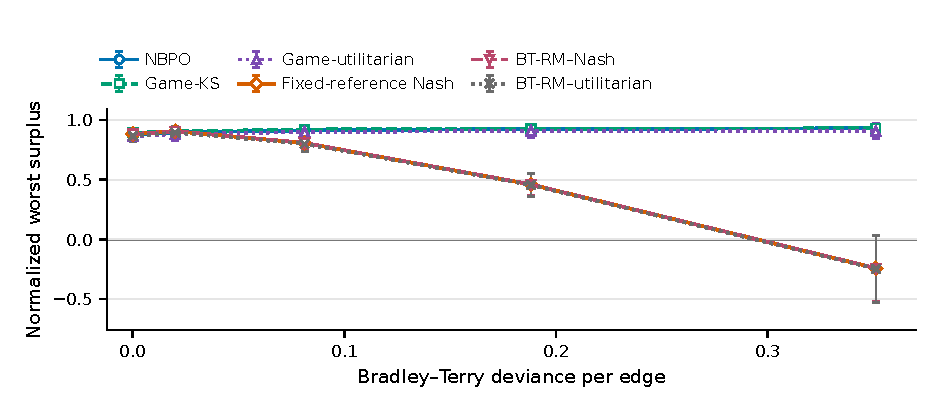
\includegraphics[width=0.78\textwidth]{figures/controlled_primary.pdf}
\caption{Controlled nontransitivity. Points show mean BT deviance and normalized worst surplus across five seeds; bars show one sample standard deviation. All six plotted methods converge. Full results and the legacy-map ablation are in Appendix~\ref{app:controlled}.}
\label{fig:controlled-gap}
\end{figure}

At the strongest perturbation, \NBPO{} reaches $0.931$ normalized worst surplus versus $-0.241$ for fixed-reference Nash and $-0.242$ for BT-RM--Nash. Game-KS and game-utilitarian also remain stable. This supports the representation claim; it does not establish Nash superiority over all aggregation rules. Independent solver residuals and robustness across constructions are reported in Appendix~\ref{app:controlled}.

\subsection{Objective-wise alignment and general capability}
\label{sec:saferlhf-exp}
\paragraph{Setup.}
We fine-tune Llama-3.1-8B-Instruct on $2{,}000$ \textsc{SafeRLHF} prompts using frozen, objective-specific preference-model ensembles. Development and held-out evaluation use $500$ and $1{,}000$ prompts. Both realizations share the solved target and response pools. The released human comparisons disagree across helpfulness and harmlessness on $24.33\%$ of held-out pairs, but contain no fully observed triangles and cannot identify within-objective human cycles. Model-predicted disagreement on generated pools is a separate quantity (Appendix~\ref{app:natural-supervision}).

\begin{table}[t]
\centering\small
\setlength{\tabcolsep}{5pt}
\caption{Teacher-defined objective evaluation on $1{,}000$ held-out prompts. Surplus is $\widehat V_k-\widehat d_k$ using common frozen comparator pools. Greedy-decoder rows do not certify stochastic-policy acceptance. The finite-pool target is a reference, not an upper bound. MSE-250 objective entries are rounded to three decimals in the execution report; its minimum is reported separately. Dashes mark unmeasured comparisons.}
\label{tab:saferlhf-main}
% Generated by scripts/render_tables.py; edit data/*.csv.
\begin{tabular}{lrrrr}
\toprule
Method & Updates & $s_{\rm help}\uparrow$ & $s_{\rm safe}\uparrow$ & $\min_k s_k\uparrow$\\
\midrule
Finite-pool target $p^\star$ & \pending & $+0.1653$ & $+0.1662$ & $+0.1653$\\
Base (greedy) & \pending & $-0.0405$ & $-0.0320$ & $-0.0405$\\
NBPO-MSE (1750) & $1750$ & $+0.1339$ & $+0.1337$ & $+0.1337$\\
NBPO-WBC (1750) & $1750$ & $+0.0738$ & $+0.0808$ & $+0.0738$\\
NBPO-MSE (250)$^\dagger$ & $250$ & $+0.119$ & $+0.125$ & $+0.1186$\\
NBPO-WBC (250)$^\dagger$ & $250$ & \pending & \pending & $+0.0569$\\
Game-utilitarian & $250$ & \pending & \pending & \pending\\
Fixed-reference Nash & $250$ & \pending & \pending & \pending\\
BT-RM--Nash & $250$ & \pending & \pending & \pending\\
PROSPER & \pending & \pending & \pending & \pending\\
MOPO & \pending & \pending & \pending & \pending\\
Game-maxmin & $250$ & \pending & \pending & \pending\\
Scalarized DPO & \pending & \pending & \pending & \pending\\
\bottomrule
\end{tabular}

\end{table}

\paragraph{Teacher-defined gains.}
MSE-250 attains worst-objective surplus $0.1186$, versus $0.1337$ for MSE-1750 and $0.0569$ for WBC-250 (Table~\ref{tab:saferlhf-main}). These are evaluations by the training preference models, relative to a stochastic-reference disagreement point. Gains concentrate on prompts where the base gives a short refusal; joint improvement alone does not identify a Nash-specific effect. Teacher truncation and this post-hoc subgroup analysis are discussed in Appendix~\ref{app:evaluation}.

\paragraph{Aggregation sensitivity.}
The Nash weights are nearly equal, $\lambda=(6.325,6.186)$. Equal weights with the same $\ell_1$ mass change the target by mean TV $0.0008$ and pairwise-target RMS $0.0034$ (Appendix~\ref{app:aggregation}). This pool provides limited target-level separation between the two rules. Policy differences and training-seed variability have not been measured; a null policy comparison would not establish equivalence.

\begin{table}[t]
\centering\scriptsize
\setlength{\tabcolsep}{3pt}
\caption{Capability and safety of the same checkpoints. Higher is better except harmful completions and benign refusals. Local reference-win proxies are not official AlpacaEval or Arena-Hard scores. Harm: HarmBench; refusal: XSTest safe prompts; tokens: Alpaca median. Measured rows currently use one seed; missing results are dashes.}
\label{tab:general-capability}
% Generated by scripts/render_tables.py; edit data/*.csv.
\begin{tabular}{lrrrrrrrr}
\toprule
Method & IFEval & GSM8K & Harm$\downarrow$ & Refusal$\downarrow$ & Alpaca & AH-hard & AH-creative & Tokens\\
\midrule
Base (greedy) & $.752$ & $.867$ & $.281$ & \pending & $.500$ & \pending & \pending & \pending\\
NBPO-MSE (1750) & $.758$ & $.864$ & $.284$ & \pending & $.419$ & \pending & \pending & \pending\\
NBPO-WBC (1750) & $.741$ & $.852$ & $.256$ & \pending & $.578$ & \pending & \pending & \pending\\
NBPO-MSE (250)$^\dagger$ & $.760$ & $.870$ & $.269$ & \pending & $.497$ & \pending & \pending & \pending\\
NBPO-WBC (250)$^\dagger$ & $.741$ & $.867$ & $.266$ & \pending & $.486$ & \pending & \pending & \pending\\
Game-utilitarian & \pending & \pending & \pending & \pending & \pending & \pending & \pending & \pending\\
Fixed-reference Nash & \pending & \pending & \pending & \pending & \pending & \pending & \pending & \pending\\
BT-RM--Nash & \pending & \pending & \pending & \pending & \pending & \pending & \pending & \pending\\
PROSPER & \pending & \pending & \pending & \pending & \pending & \pending & \pending & \pending\\
MOPO & \pending & \pending & \pending & \pending & \pending & \pending & \pending & \pending\\
Game-maxmin & \pending & \pending & \pending & \pending & \pending & \pending & \pending & \pending\\
Scalarized DPO & \pending & \pending & \pending & \pending & \pending & \pending & \pending & \pending\\
\bottomrule
\end{tabular}

\end{table}

\paragraph{External evaluation.}
MSE-250 obtains IFEval $0.760$, GSM8K $0.870$, and harmful-completion rate $0.269$, compared with $0.752$, $0.867$, and $0.281$ for the base. Its Alpaca local win rate is $0.497$; these point estimates do not establish equivalence or overall superiority. WBC-1750 has a higher local win rate ($0.578$) despite lower teacher-defined surplus. Independent objective evaluation, policy-seed repeats, and a scalarization sweep are required to assess empirical nondominance (Appendix~\ref{app:pareto-evaluation}).

\subsection{Projection and training schedule}
\label{sec:neural-general}
We compare canonical regression with WBC under matched data and policy-token exposure. The original comparison uses $1750$ updates. After inspecting its development trajectories, we declared separate $250$-update follow-ups, each with its own cosine schedule. They are development-informed runs, not truncated long runs or a fully prospective $2\times2$ study.

\begin{table}[t]
\centering\small
\setlength{\tabcolsep}{5pt}
\caption{Target realization on $500$ development prompts, one seed. Each horizon has its own cosine schedule; $250$-update runs are development-informed follow-ups. Pool KL is $D_{\rm KL}(p^\star\|\widehat p_\theta)$ on sampled support; the reference value is $0.7879$. Full diagnostics are in Appendix~\ref{app:solver-neural}.}
\label{tab:repaired-realization}
% Generated by scripts/render_tables.py; edit data/*.csv.
\begin{tabular}{lrrrrrr}
\toprule
Projection & Horizon & nMSE & Sign & Pearson & Pool KL$\downarrow$ & GPU-h\\
\midrule
MSE & $1750$ & $1.418$ & $0.693$ & $0.415$ & $1.2131$ & $7.48$\\
WBC & $1750$ & $13.070$ & $0.486$ & $-0.152$ & $6.0634$ & $6.78$\\
MSE$^\dagger$ & $250$ & $0.690$ & $0.702$ & $0.588$ & $0.6204$ & $2.20$\\
WBC$^\dagger$ & $250$ & $0.780$ & $0.687$ & $0.492$ & $0.6875$ & $2.08$\\
\bottomrule
\end{tabular}

\end{table}

Both short runs pass the existing target-fit thresholds: nMSE $<0.90$, sign $>0.65$, and positive Pearson and Spearman correlations. MSE-250 also reduces finite-pool KL from $0.7879$ to $0.6204$. MSE-1750 has positive correlation but increases KL; it already fails the original nMSE threshold. Thus correlation alone is insufficient, while no gate false positive is demonstrated here. These are importance-reweighted pool distributions, not full-policy KLs. Update count, exposure, and learning-rate trajectory change together, so horizon is not isolated as the sole cause.
\section{Related Work}
\label{sec:related}
\paragraph{General pairwise preferences.}
NLHF and its scalable variants optimize directly against general pairwise preference models rather than fitting scalar rewards \citep{munos2024nash,wu2025sppo,zhang2025iterative,calandriello2024online,rosset2024direct,zhou2025egpo}. Blackwell-style methods extend this view to vector-valued feedback and target sets \citep{blackwell1956analog,bhatia2020multicriteria}. PROSPER introduces a maximum-entropy Blackwell winner with a scalable single-policy update and an inner worst-case choice over objective weights and opponents \citep{zhang2026prosper}. \NBPO{} instead keeps one regularized game value per objective and applies Nash bargaining across the improvements over a shared fallback.

\paragraph{Reward-based multi-objective alignment.}
MODPO, Rewarded Soups, and Panacea expose user-specified trade-offs through scalarization, policy interpolation, or preference conditioning \citep{zhou2024beyond,rame2023rewarded,zhong2024panacea}. MaxMin-RLHF and RMOD optimize weakest-objective criteria, while MOPO designates a primary objective and lower-bound constraints for the others \citep{chakraborty2024maxmin,son2026rmod,agnihotri2026mopo}. These methods are important empirical baselines because they explicitly fit or use scalar objective rewards, whereas \NBPO{} learns from general pairwise feedback without assuming that each objective is transitive.

\paragraph{Social choice and bargaining.}
The Nash solution and its Pareto, uniqueness, and affine-invariance properties are classical \citep{nash1950}. Social-choice work argues that alignment should state its aggregation rule explicitly \citep{conitzer2024social}. Multi-party RLHF studies utilitarian, Nash, and leximin welfare over party-specific learned rewards and separately considers reward-free von Neumann solutions \citep{zhong2024nashwelfare}; Nash bargaining has also been used to combine task gradients in multi-task learning \citep{navon2022nashmtl}. Our contribution is not a new bargaining axiom, but a formulation and practical optimizer for applying the classical Nash rule to policy-dependent objective-wise preference-game values.

\section{Conclusion and Limitations}
\label{sec:conclusion}
\NBPO{} combines adaptive preference-game values with Nash bargaining over reference-relative improvements. A constrained proximal formulation yields a direct finite-pool solver and an $O(1/T)$ exact-population guarantee. Controlled experiments support adaptive game representations. Short-schedule 8B regression improves target fit and teacher-defined outcomes with near-base capability point estimates. An aggregation advantage and empirical Pareto optimality remain unestablished. Teacher truncation, refusal-concentrated gains, development-informed schedules, and a single policy seed limit the conclusions. Joint improvement need not be feasible, and population game values provide no per-prompt safety guarantee.

\subsection*{AI use statement}
In this work, generative AI tools were used to critique the problem formulation, assist with mathematical derivations and proof presentation, propose experimental checks, and edit manuscript text. The authors are responsible for independently verifying every theorem, citation, implementation, empirical result, and disclosure in the final submission.

\subsection*{Ethics statement}
This work studies aggregation rules for language-model alignment, including harmlessness as one objective. Improvement in a game value is not an absolute safety certificate. Safety-critical deployment should retain hard constraints and independent safety evaluations in addition to the bargaining objective.

\subsection*{Reproducibility statement}
Algorithm~\ref{alg:nbpo} distinguishes the population proximal problem, the numerically solved finite-pool inner problem, and its neural projection. Appendix~\ref{app:proofs} contains the dual and convergence proofs; Appendices~\ref{app:controlled}--\ref{app:evaluation} specify constructions, supervision, hyperparameters, diagnostics, and evaluation protocols. The submission package should include candidate pools, preference tensors, dual traces, solver residuals, per-seed outputs, and the code and configurations required to reproduce the reported results.

\bibliography{iclr2027_conference}
\bibliographystyle{iclr2027_conference}

\appendix

\section{Proofs}
\label{app:proofs}

\subsection{Proof of Proposition~\ref{prop:game-structure}}
\label{app:proof-game-structure}
For a fixed comparator $\nu$, define
\[
\mathcal J_{k,\nu}(\pi)
:=
J_k(\pi,\nu)
+
\beta_k\E_{x\sim\D}
\KL\!\left(\nu(\cdot\mid x)\,\|\,\piref(\cdot\mid x)\right).
\]
The first term is linear in $\pi$ and the second does not depend on $\pi$, so $\mathcal J_{k,\nu}$ is affine. The pointwise minimum of affine functions is concave; hence $V_{k,\beta_k}$ is concave. Since $|\Delta_k|\le1/2$,
\[
|V_{k,\beta_k}(\pi)-V_{k,\beta_k}(\pi')|
\le
\frac12\E_{x\sim\D}
\|\pi(\cdot\mid x)-\pi'(\cdot\mid x)\|_1,
\]
which also proves continuity.

For $\beta_k>0$, the inner minimization separates across prompts. Fix $x$ and abbreviate $m(z)=m_k^\pi(z\mid x)$. The prompt-wise problem is
\[
\min_{\nu\in\Delta(\Y_x)}
\sum_z\nu(z)m(z)
+
\beta_k\sum_z\nu(z)
\log\frac{\nu(z)}{\piref(z\mid x)}.
\]
The first-order condition under $\sum_z\nu(z)=1$ gives
\[
\nu(z)\propto\piref(z\mid x)\exp\{-m(z)/\beta_k\},
\]
which yields \eqref{eq:regularized-opponent}; substituting it back yields \eqref{eq:soft-value}. The KL term makes the minimizer unique. Danskin's theorem therefore gives, for every feasible direction $h$ satisfying $\sum_yh(y\mid x)=0$,
\[
D V_{k,\beta_k}(\pi)[h]
=
\E_{x\sim\D}\sum_y h(y\mid x)
\E_{z\sim\nu^\star_{k,\pi}(\cdot\mid x)}
\Delta_k(y,z\mid x).
\]
Thus the coordinate derivative is
\[
\left[\nabla_\pi V_{k,\beta_k}(\pi)\right]_{x,y}
=
\D(x)Q_k^\pi(y\mid x),
\]
proving \eqref{eq:game-gradient}.

\subsection{Connection to the Fixed-Reference}
\label{app:anchor-limit}
This subsection gives a finite-action illustration at the unregularized endpoint $\beta=0$. It is not used in Assumption~\ref{ass:joint}, the full-support analysis, or the finite-temperature experiments.

Define the fixed-reference improvement
\begin{equation}
a_k(\pi)=J_k(\pi,\piref)=P_k(\pi\succ\piref)-\tfrac12.
\label{eq:anchor-margin}
\end{equation}
Skew-symmetry gives $a_k(\piref)=0$.

\paragraph{Full cyclic example.}
For one prompt, let $\piref=\delta_r$, where $\delta_y$ is the deterministic
policy that always outputs $y$. Suppose $A$, $B$, and $C$ each beat $r$
with probability $0.75$ and form the deterministic cycle
\[
A\succ B,\qquad B\succ C,\qquad C\succ A.
\]
Both
\[
\pi_{\rm pure}=\delta_A
\qquad\text{and}\qquad
\pi_{\rm mix}=\frac{\delta_A+\delta_B+\delta_C}{3}
\]
have the same fixed-reference improvement,
\[
a(\pi_{\rm pure})
=
a(\pi_{\rm mix})
=
0.75-\frac12
=
0.25.
\]

Their worst-opponent values are nevertheless different. For the pure
policy, response $C$ defeats $A$ deterministically, so
\[
V_0(\pi_{\rm pure})
=
\min_{\nu} J(\pi_{\rm pure},\nu)
=
J(\delta_A,\delta_C)
=
-\frac12.
\]

For the uniform mixture, consider first the pure opponent $\delta_A$.
The mixture outputs $A$, $B$, and $C$ with equal probability. Against
$A$, these responses respectively tie, lose, and win, giving centered
payoffs $0$, $-1/2$, and $+1/2$. Hence
\[
J(\pi_{\rm mix},\delta_A)
=
\frac13
\left(
0-\frac12+\frac12
\right)
=
0.
\]
By symmetry,
\[
J(\pi_{\rm mix},\delta_B)
=
J(\pi_{\rm mix},\delta_C)
=
0.
\]
Against the reference,
\[
J(\pi_{\rm mix},\delta_r)=0.25,
\]
because every response in the mixture beats $r$ with probability $0.75$.
Since $J(\pi_{\rm mix},\nu)$ is linear in $\nu$, no mixed opponent can
achieve a value below the minimum over these pure opponents. Therefore
\[
V_0(\pi_{\rm mix})
=
\min_{\nu}J(\pi_{\rm mix},\nu)
=
\min\{0,0,0,0.25\}
=
0.
\]

Finally, the reference itself has
\[
V_0(\piref)
=
\min_{\nu}J(\delta_r,\nu)
=
-0.25,
\]
since $r$ loses to each of $A$, $B$, and $C$ with probability $0.75$.
Thus
\[
\begin{array}{c|ccc}
& a(\pi) & V_0(\pi) & V_0(\pi)-V_0(\piref)\\
\hline
\pi_{\rm pure} & 0.25 & -0.50 & -0.25\\
\pi_{\rm mix}  & 0.25 & 0     &  0.25
\end{array}
\]
The fixed reference therefore assigns the two policies the same score,
even though the pure policy is fully exploitable by one response whereas
the balanced mixture guarantees an average tie against every response
in the cycle.

\subsection{Policy-Induced Nash Bargaining and Classical Consequences}
\label{app:nash-properties}
We prove Proposition~\ref{prop:nash-outcome}. Since $\Pi$ is compact and each $V_{k,\beta_k}$ is continuous, $V_{\boldsymbol\beta}(\pi)$ is bounded. The definition of $\G_{\boldsymbol\beta}$ then implies boundedness. Closedness follows by taking any convergent sequence $v_n\in\G_{\boldsymbol\beta}$, choosing policies $\pi_n$ with $d\le v_n\le V_{\boldsymbol\beta}(\pi_n)$, extracting a convergent policy subsequence, and applying continuity. Downward closure is immediate from the definition.

For convexity, take $v^1,v^2\in\G_{\boldsymbol\beta}$ with witnesses $\pi_1,\pi_2$. Objective-wise concavity from Proposition~\ref{prop:game-structure} gives, for $\alpha\in[0,1]$,
\[
V_{\boldsymbol\beta}(\alpha\pi_1+(1-\alpha)\pi_2)
\ge
\alpha V_{\boldsymbol\beta}(\pi_1)+(1-\alpha)V_{\boldsymbol\beta}(\pi_2)
\]
componentwise, so $\alpha v^1+(1-\alpha)v^2\in\G_{\boldsymbol\beta}$. Assumption~\ref{ass:joint} provides a point strictly above $d$, proving nondegeneracy.

For any $v\in\G_{\boldsymbol\beta}$ with $v>d$, some policy $\pi$ satisfies $v\le V_{\boldsymbol\beta}(\pi)$. Since the Nash objective is coordinatewise increasing,
\[
\sum_k\log(v_k-d_k)
\le
\sum_k\log\bigl(V_{k,\beta_k}(\pi)-d_k\bigr)
=F(\pi).
\]
Conversely, every $\pi\in\Pi_+$ induces a feasible value vector $V_{\boldsymbol\beta}(\pi)$. Hence \eqref{eq:nash-welfare} realizes the classical Nash solution over $(\G_{\boldsymbol\beta},d)$.

The remaining statements are standard Nash-bargaining consequences, but we record the short arguments for completeness. Since the log objective tends to $-\infty$ when any surplus approaches zero, every optimizer lies strictly above $d$. Coordinatewise monotonicity implies Pareto optimality. Strict concavity of $\sum_k\log s_k$ over value vectors implies that all optimal policies induce the same surplus, hence the same game-value vector, although the policy itself can be nonunique.

Finally, under independent positive affine transformations
\[
V_k'(\pi)=c_kV_k(\pi)+b_k,
\qquad
d_k'=c_kd_k+b_k,
\qquad c_k>0,
\]
the transformed surplus is $s_k'(\pi)=c_ks_k(\pi)$ and
\[
\sum_k\log s_k'(\pi)
=
\sum_k\log s_k(\pi)+\sum_k\log c_k.
\]
The added term is independent of $\pi$, so the optimizer set is unchanged.

\begin{table}[htbp]
\centering\footnotesize
\setlength{\tabcolsep}{4.2pt}
\caption{Classical population guarantees of common aggregation rules under joint improvement. The Nash row follows from the standard bargaining solution; the other rows are supported by the finite counterexamples below.}
\label{tab:rule-guarantees}
\begin{tabular}{lcccc}
\toprule
rule & strict IR & Pareto optimal & unique value & affine invariant\\
\midrule
positive-weight utilitarian & no & yes & no & no\\
absolute maxmin & no & no & no & no\\
surplus maxmin & yes & no & no & no\\
Nash bargaining & yes & yes & yes & yes\\
\bottomrule
\end{tabular}
\end{table}

\subsection{Counterexamples for Alternative Aggregation Rules}
\label{app:rule-witnesses}

The positive guarantees in Table~\ref{tab:rule-guarantees} follow
directly from the corresponding objectives. Because $w_k>0$, the
positive-weight utilitarian objective $\sum_k w_k V_k(\pi)$ is strictly
increasing in every game-value coordinate, so none of its optimizers can
be Pareto dominated. Under Assumption~\ref{ass:joint}, surplus maxmin
also attains a strictly positive minimum surplus because a jointly
improving policy exists. The examples below establish the guarantees
that can fail for the alternative rules.

All examples use three responses, so a policy is a probability vector
$\pi=(\pi_1,\pi_2,\pi_3)\in\Delta_3$, and use the uniform reference
$\piref=(1/3,1/3,1/3)$. For objective $k$, $\Delta_k$ is the skew-symmetric
pairwise payoff matrix: $(\Delta_k)_{ij}$ is the centered preference margin of response
$i$ against response $j$. At $\beta_k=0$,
\[
V_k(\pi)
=
\min_j(\pi^\top \Delta_k)_j,
\qquad
d_k=V_k(\piref),
\qquad
s_k(\pi)=V_k(\pi)-d_k.
\]
Thus $\pi^\top \Delta_k$ contains the expected payoff of $\pi$ against each
pure opponent, and $V_k(\pi)$ is its smallest coordinate.

Because each $V_k$ is the minimum of linear functions, the optimizers
below are obtained from small linear programs. For example,
equal-weight utilitarian optimization can be written as
\[
\max_{\pi,t_1,t_2}\ t_1+t_2
\quad\text{s.t.}\quad
t_k\le(\pi^\top \Delta_k)_j
\ \ \forall k,j,\qquad
\pi\in\Delta_3.
\]
Absolute maxmin uses one variable $t$ with
$t\le(\pi^\top \Delta_k)_j$, while surplus maxmin uses
$t+d_k\le(\pi^\top \Delta_k)_j$ for every $k,j$.

\paragraph{Utilitarian failure of strict improvement.}
Let
\[
\Delta_1=
\begin{pmatrix}
0&-1/2&-1/2\\
1/2&0&-1/2\\
1/2&1/2&0
\end{pmatrix},
\qquad
\Delta_2=
\begin{pmatrix}
0&-1/2&1/4\\
1/2&0&-1/2\\
-1/4&1/2&0
\end{pmatrix}.
\]
For the uniform reference,
\[
\piref^\top \Delta_1=(1/3,0,-1/3),
\qquad
\piref^\top \Delta_2=(1/12,0,-1/12),
\]
and hence
\[
d=(-1/3,-1/12).
\]

First, joint improvement is feasible. The policy
\[
\bar\pi=(1/4,1/4,1/2)
\]
is only a feasibility witness; it gives
\[
\bar\pi^\top \Delta_1=(3/8,1/8,-1/4),
\qquad
\bar\pi^\top \Delta_2=(0,1/8,-1/16).
\]
Therefore
\[
V(\bar\pi)=(-1/4,-1/16),
\qquad
s(\bar\pi)
=
V(\bar\pi)-d
=
(1/12,1/48)>0.
\]

In contrast, solving the equal-weight utilitarian problem
$\max_\pi V_1(\pi)+V_2(\pi)$ gives
\[
\pi_{\rm U}=(0,1/5,4/5).
\]
For this policy,
\[
\pi_{\rm U}^\top \Delta_1=(1/2,2/5,-1/10),
\qquad
\pi_{\rm U}^\top \Delta_2=(-1/10,2/5,-1/10),
\]
so
\[
V(\pi_{\rm U})=(-1/10,-1/10),
\qquad
s(\pi_{\rm U})
=
(7/30,-1/60).
\]
Thus joint improvement is possible, yet a utilitarian optimum falls
below the fallback on objective~2.

\paragraph{Absolute-maxmin failure of strict improvement.}
Let
\[
\Delta_1=
\begin{pmatrix}
0&-1/2&1/4\\
1/2&0&1/2\\
-1/4&-1/2&0
\end{pmatrix},
\qquad
\Delta_2=
\begin{pmatrix}
0&1/4&-1/2\\
-1/4&0&1/2\\
1/2&-1/2&0
\end{pmatrix}.
\]
Again,
\[
d=(-1/3,-1/12).
\]
Joint improvement is feasible, as witnessed by
\[
\bar\pi=(1/3,7/15,1/5),
\]
for which
\[
V(\bar\pi)=(-4/15,-1/60)
\]
and therefore
\[
s(\bar\pi)=(1/15,1/15)>0.
\]

Absolute maxmin instead solves
\[
\max_{\pi}\min\{V_1(\pi),V_2(\pi)\},
\]
whose linear-program solution is
\[
\pi_{\rm AM}=(0,4/5,1/5).
\]
For this policy,
\[
\pi_{\rm AM}^\top \Delta_1=(7/20,-1/10,2/5),
\qquad
\pi_{\rm AM}^\top \Delta_2=(-1/10,-1/10,2/5),
\]
so
\[
V(\pi_{\rm AM})=(-1/10,-1/10)
\]
and
\[
s(\pi_{\rm AM})
=
(7/30,-1/60).
\]
Thus absolute maxmin maximizes the smallest \emph{absolute} game value
while allowing objective~2 to fall below its own fallback.

\paragraph{A Pareto-dominated surplus-maxmin optimum.}
Let
\[
\Delta_1=
\begin{pmatrix}
0&-1/2&1/2\\
1/2&0&1/2\\
-1/2&-1/2&0
\end{pmatrix},
\qquad
\Delta_2=
\begin{pmatrix}
0&0&1/2\\
0&0&1/2\\
-1/2&-1/2&0
\end{pmatrix}.
\]
The uniform reference gives
\[
d=(-1/3,-1/6).
\]
For objective~2, no policy can achieve $V_2(\pi)>0$, while every mixture
supported on the first two responses achieves $V_2(\pi)=0$.
Consequently,
\[
s_2(\pi)\le 1/6
\]
for every policy, so the optimal surplus-maxmin value cannot exceed
$1/6$.

The two policies
\[
\pi_c=(1/3,2/3,0),
\qquad
\pi_e=(0,1,0)
\]
satisfy
\[
V(\pi_c)=(-1/6,0),
\qquad
s(\pi_c)=(1/6,1/6),
\]
and
\[
V(\pi_e)=(0,0),
\qquad
s(\pi_e)=(1/3,1/6).
\]
Both therefore maximize
\[
\min_k s_k(\pi)
\]
at $1/6$. However,
\[
s(\pi_e)>s(\pi_c)
\]
in the first coordinate and is equal in the second, so
$\pi_e$ Pareto dominates $\pi_c$. Thus the surplus-maxmin optimizer set
can contain Pareto-dominated policies.

\subsection{Dual Derivation and Regression Fixed Point}
\label{app:prox-dual}
For multipliers $\lambda_k\ge0$, the Lagrangian of \eqref{eq:prox-subproblem} is
\[
\mathcal L_t(\pi,u,\lambda)
=
\sum_k\log u_k
+
\sum_k\lambda_k\bigl(s_k(\pi)-u_k\bigr)
-
\eta_t^{-1}D(\pi\|\pi_t).
\]
For fixed $\lambda_k>0$, maximizing $\log u_k-\lambda_ku_k$ gives $u_k=1/\lambda_k$ and value $-\log\lambda_k-1$; if $\lambda_k=0$, the maximum is unbounded. Substitution yields \eqref{eq:prox-dual}, and the remaining maximization over $\pi$ is \eqref{eq:weighted-policy}. Uniqueness of that maximizer and Danskin's theorem yield \eqref{eq:dual-gradient}.

Assumption~\ref{ass:joint} provides strict feasibility: choose $\bar\pi$ with $s_k(\bar\pi)>0$ and $0<\bar u_k<s_k(\bar\pi)$. Slater's condition therefore gives strong duality. Stationarity in $u_k$ gives
\[
\lambda_{t+1,k}=\frac{1}{u_{t+1,k}}>0,
\]
and complementary slackness then forces $u_{t+1,k}=s_k(\pi_{t+1})$. This proves Proposition~\ref{prop:prox-dual}.

\paragraph{Dual step used as a fallback.}
Stationarity $\widehat s_k(p_t^\star(\lambda))=1/\lambda_k$ can also be approached by projected subgradient \emph{descent} on the dual --- the update below subtracts the dual gradient, and the dual of the concave inner problem is minimized over $\lambda$ ---
\begin{equation}
\lambda^{(m+1)}
=
\Pi_{\Lambda}\!\left[
\lambda^{(m)}-
\gamma_m\left(
\widehat s\!\left(p_t^\star(\lambda^{(m)})\right)
-(\lambda^{(m)})^{-1}
\right)
\right],
\label{eq:dual-update}
\end{equation}
where $\gamma_m>0$ is the dual step size, $\Pi_{\Lambda}$ is Euclidean projection onto $\Lambda=[\lambda_{\min},\lambda_{\max}]^K$ with $0<\lambda_{\min}<\lambda_{\max}$, and the inverse is elementwise. On the pools reported here this iteration stalls at a projected KKT residual near $10^{-2}$ after $3000$ steps, whereas the root solve reaches $10^{-9}$ in tens of inner solves; no reported result uses \eqref{eq:dual-update}.

\paragraph{What the projected certificate certifies.}
Both the root solve and the fallback act on the box $\Lambda=[\lambda_{\min},\lambda_{\max}]^K$, so the residual we report is the projected KKT residual of the \emph{box-constrained} dual. That residual certifies the original problem only when the box is inactive at the returned $\lambda$: on an active bound the projection can annihilate a genuine stationarity violation, and a small number then certifies nothing. We therefore report bound activity alongside every residual and treat a run with an active bound as uncertified rather than converged. In the runs reported here the multipliers are interior by a wide margin --- on the \textsc{SafeRLHF} pool, $\Lambda=[10^{-3},10^{3}]^2$ and the solved $\lambda=(6.33,6.19)$ sit at least two decades from either bound in $\log_{10}\lambda$ --- and the stationarity residual recomputed independently from the returned policy is $6.7\times10^{-11}$.

\paragraph{Finite-pool optimality and neural projection.}
Fix $\lambda$ and let $\pi_t^\star(\lambda)$ solve \eqref{eq:weighted-policy}. First-order optimality gives, for every prompt and response pair in the support,
\begin{equation}
h_t(\pi_t^\star(\lambda);x,y,y')
=
\eta_t\sum_k\lambda_k
\left(
Q_k^{\pi_t^\star(\lambda)}(y\mid x)
-
Q_k^{\pi_t^\star(\lambda)}(y'\mid x)
\right).
\label{eq:prox-pairwise-kkt}
\end{equation}
The direct finite-pool program \eqref{eq:direct-inner} is the sampled analogue of this strictly concave problem. Its normalized optimizer determines all finite-pool log-probability differences, so \eqref{eq:finite-target-logratio} is identified without computing a language-model normalizer. Equation~\eqref{eq:finite-target-identity} is the corresponding finite-pool KKT identity and is checked numerically before an artifact is accepted. With a full-support pair proposal, zero regression error implies
\[
\widetilde p_{\theta,x}(i)
=\frac{p_{t,x}(i)\,\pi_\theta(y_{x,i}\mid x)/\pi_t(y_{x,i}\mid x)}
{\sum_j p_{t,x}(j)\,\pi_\theta(y_{x,j}\mid x)/\pi_t(y_{x,j}\mid x)}
=p_{t,x}^\star(i).
\]
This is an importance-reweighted occurrence measure, not the raw LM probabilities normalized within the pool. It does not guarantee finite-sample optimization or generalization of the neural model.

\subsection{Last-Iterate Convergence}
\label{app:convergence}
\begin{theorem}[Last-iterate convergence]
\label{thm:last-iterate}
Under Assumption~\ref{ass:joint}, let $\pi^\star$ maximize \eqref{eq:nash-welfare}, set $\pi_0=\piref$, and solve \eqref{eq:prox-subproblem} exactly at every outer iteration with arbitrary $\eta_t>0$. Then $F(\pi_{t+1})\ge F(\pi_t)$ for $t\ge1$, and for every $T\ge1$,
\begin{equation}
F(\pi^\star)-F(\pi_T)
\le
\frac{D(\pi^\star\|\piref)}{\sum_{t=0}^{T-1}\eta_t}.
\label{eq:last-iterate-rate}
\end{equation}
\end{theorem}

Work throughout in the $\D$-weighted geometry: pair functions of $(x,y)$ by $\langle f,g\rangle_\D=\E_{x\sim\D}\sum_yf(x,y)g(x,y)$, and let $h$ be the \emph{prompt-wise} negative entropy $h(\pi)(x)=\sum_y\pi(y\mid x)\log\pi(y\mid x)$, whose gradient at $(x,y)$ is $1+\log\pi(y\mid x)$. Its Bregman divergence in that geometry is exactly $D(\pi\|\pi_t)=\E_{x\sim\D}\KL(\pi(\cdot\mid x)\|\pi_t(\cdot\mid x))$. The prompt expectation enters once, through the pairing, and is not also carried inside $h$. Because the objective is increasing in $u$, the policy part of \eqref{eq:prox-subproblem} is equivalently
\begin{equation}
\pi_{t+1}
\in
\arg\max_{\pi\in\Pi_+}
\left\{F(\pi)-\frac1{\eta_t}D(\pi\|\pi_t)\right\}.
\label{eq:implicit-prox}
\end{equation}
The feasible set is nonempty by Assumption~\ref{ass:joint}, and $F(\pi)\to-\infty$ as any surplus approaches zero. Thus the maximizer exists in $\Pi_+$ even when the center $\pi_t$ is the reference $\piref\notin\Pi_+$. Because $\pi_t$ has full support and the remaining objective has finite directional derivatives at an interior surplus point, the inward derivative of $-D(\pi\|\pi_t)$ excludes zero-probability coordinates. Induction therefore gives a full-support, positive-surplus $\pi_{t+1}$.

Let $g_{t+1}$ be a supergradient of $F$ at $\pi_{t+1}$. First-order optimality of \eqref{eq:implicit-prox} and concavity of $F$ imply, for every $\pi\in\Pi_+$,
\begin{align}
F(\pi)-F(\pi_{t+1})
&\le \langle g_{t+1},\pi-\pi_{t+1}\rangle_\D\\
&\le\frac1{\eta_t}
\left\langle\nabla h(\pi_{t+1})-\nabla h(\pi_t),
\pi-\pi_{t+1}\right\rangle_\D\\
&=\frac1{\eta_t}
\left[
D(\pi\|\pi_t)-D(\pi\|\pi_{t+1})-D(\pi_{t+1}\|\pi_t)
\right].
\label{eq:prox-three-point}
\end{align}
For $t\ge1$, $\pi_t$ is feasible in the next subproblem. Comparing the optimum with $\pi_t$ gives
\begin{equation}
F(\pi_{t+1})-\frac{1}{\eta_t}D(\pi_{t+1}\|\pi_t)
\ge F(\pi_t),
\label{eq:prox-monotone}
\end{equation}
so the objective values are nondecreasing from $\pi_1$ onward.

Set $\pi=\pi^\star$ in \eqref{eq:prox-three-point}, multiply by $\eta_t$, and sum from $t=0$ to $T-1$:
\begin{equation}
\sum_{t=0}^{T-1}\eta_t
\big(F(\pi^\star)-F(\pi_{t+1})\big)
\le
D(\pi^\star\|\piref).
\label{eq:prox-telescope}
\end{equation}
Because the gaps are nonincreasing, the left-hand side is at least
$\big(\sum_t\eta_t\big)(F(\pi^\star)-F(\pi_T))$, which proves \eqref{eq:last-iterate-rate}.

\begin{corollary}[Convergence of the surplus profile]
\label{cor:surplus-convergence}
Under the conditions of Theorem~\ref{thm:last-iterate}, let
$s^\star=s(\pi^\star)$ denote the unique surplus vector induced by a
Nash-optimal policy. Then
\begin{equation}
\|s(\pi_T)-s^\star\|_2^2
\le
\frac{2D(\pi^\star\|\piref)}
{\sum_{t=0}^{T-1}\eta_t}.
\label{eq:last-iterate-surplus}
\end{equation}
Hence a constant proximal step gives
$\|s(\pi_T)-s^\star\|_2=O(T^{-1/2})$.
\end{corollary}

\begin{proof}
This is a stronger consequence of Nash-welfare convergence rather than a
separate requirement for the NBPO update. For every objective,
$V_k(\pi)\in[-1/2,1/2]$, and
$d_k=V_k(\piref)\le0$ because $\nu=\piref$ is feasible and
$J_k(\piref,\piref)=0$. Hence every positive surplus is at most one. On
$(0,1]^K$, the function
$G(s)=\sum_k\log s_k$ is $1$-strongly concave in Euclidean norm.
Proposition~\ref{prop:nash-outcome} implies that all Nash-optimal policies induce the
same game-value vector, and therefore the same surplus vector $s^\star$.
First-order optimality over the convex comprehensive surplus set induced by
\eqref{eq:comprehensive-hull} gives
\begin{equation}
G(s^\star)-G(s)
\ge
\frac12\|s-s^\star\|_2^2.
\label{eq:surplus-strong-concavity}
\end{equation}
Applying this inequality to $s=s(\pi_T)$ and using
\eqref{eq:last-iterate-rate} proves \eqref{eq:last-iterate-surplus}.
\end{proof}

\section{Controlled Benchmark: Construction and Full Results}
\label{app:controlled}
\paragraph{Feasibility-preserving construction.}
For every seed we form a transitive base matrix and an odd-cardinality circulant skew-symmetric perturbation. Zero row sums keep the uniform reference disagreement invariant, while bisection selects the cycle magnitude so that $\rho^\star=\max_\pi\min_k s_k(\pi)$ stays close to a target margin. We reject invalid probabilities rather than clip matrix entries. The resulting panel increases BT deviance from approximately $2.7\times10^{-4}$ to $0.351$ while retaining positive joint improvement in every instance. All policies are evaluated under the same adaptive-game values, not their method-native scales.

\begin{table*}[t]
\centering\scriptsize
\setlength{\tabcolsep}{2.1pt}
\caption{Full controlled results over five seeds under the common adaptive-game evaluator. Residuals are method-specific; the legacy map is a non-convergence ablation.}
\label{tab:controlled-full}
\begin{tabular}{lrrrrrr}
\toprule
method & min surplus & sd & $\min s/\rho^\star$ & sd & exploitability & inner resid.\\
\midrule
\multicolumn{7}{l}{\textit{$\alpha=0.00$, $\rho^\star=0.0300$, BT dev.\ $=0.0003$}}\\
\quad \NBPO{} direct & $+0.0264$ & $0.0011$ & $0.881$ & $0.037$ & $0.0687$ & $2\times10^{-12}$\\
\quad Game-KS & $+0.0268$ & $0.0005$ & $0.893$ & $0.017$ & $0.0685$ & $10^{-9}$\\
\quad Game-util. & $+0.0260$ & $0.0014$ & $0.866$ & $0.048$ & $0.0688$ & $3\times10^{-10}$\\
\quad Fixed-ref.\ Nash & $+0.0265$ & $0.0011$ & $0.883$ & $0.036$ & $0.0688$ & $0$\\
\quad BT-RM--Nash & $+0.0265$ & $0.0011$ & $0.883$ & $0.036$ & $0.0688$ & $0$\\
\quad BT-RM--util. & $+0.0260$ & $0.0014$ & $0.867$ & $0.047$ & $0.0689$ & $0$\\
\quad legacy $R$-step$^\dagger$ & $+0.0252$ & $0.0012$ & $0.840$ & $0.041$ & $0.0675$ & $5\times10^{-10}$\\
\addlinespace
\multicolumn{7}{l}{\textit{$\alpha=0.25$, $\rho^\star=0.0300$, BT dev.\ $=0.0202$}}\\
\quad \NBPO{} direct & $+0.0269$ & $0.0013$ & $0.897$ & $0.044$ & $0.1091$ & $10^{-7}$\\
\quad Game-KS & $+0.0272$ & $0.0007$ & $0.905$ & $0.025$ & $0.1088$ & $10^{-7}$\\
\quad Game-util. & $+0.0265$ & $0.0017$ & $0.883$ & $0.058$ & $0.1094$ & $4\times10^{-8}$\\
\quad Fixed-ref.\ Nash & $+0.0272$ & $0.0012$ & $0.907$ & $0.040$ & $0.1197$ & $0$\\
\quad BT-RM--Nash & $+0.0272$ & $0.0012$ & $0.907$ & $0.040$ & $0.1197$ & $0$\\
\quad BT-RM--util. & $+0.0269$ & $0.0015$ & $0.895$ & $0.049$ & $0.1198$ & $0$\\
\quad legacy $R$-step$^\dagger$ & $+0.0258$ & $0.0014$ & $0.860$ & $0.046$ & $0.1063$ & $7\times10^{-1}$\\
\addlinespace
\multicolumn{7}{l}{\textit{$\alpha=0.50$, $\rho^\star=0.0300$, BT dev.\ $=0.0813$}}\\
\quad \NBPO{} direct & $+0.0274$ & $0.0013$ & $0.914$ & $0.044$ & $0.1454$ & $2\times10^{-6}$\\
\quad Game-KS & $+0.0276$ & $0.0007$ & $0.921$ & $0.023$ & $0.1450$ & $2\times10^{-7}$\\
\quad Game-util. & $+0.0270$ & $0.0017$ & $0.900$ & $0.057$ & $0.1458$ & $2\times10^{-7}$\\
\quad Fixed-ref.\ Nash & $+0.0243$ & $0.0018$ & $0.809$ & $0.059$ & $0.1945$ & $0$\\
\quad BT-RM--Nash & $+0.0243$ & $0.0018$ & $0.809$ & $0.058$ & $0.1945$ & $0$\\
\quad BT-RM--util. & $+0.0240$ & $0.0019$ & $0.800$ & $0.064$ & $0.1947$ & $0$\\
\quad legacy $R$-step$^\dagger$ & $+0.0025$ & $0.0044$ & $0.082$ & $0.147$ & $0.1981$ & $10\times10^{-1}$\\
\addlinespace
\multicolumn{7}{l}{\textit{$\alpha=0.75$, $\rho^\star=0.0300$, BT dev.\ $=0.1882$}}\\
\quad \NBPO{} direct & $+0.0278$ & $0.0013$ & $0.926$ & $0.042$ & $0.1693$ & $8\times10^{-6}$\\
\quad Game-KS & $+0.0278$ & $0.0005$ & $0.928$ & $0.018$ & $0.1692$ & $8\times10^{-7}$\\
\quad Game-util. & $+0.0273$ & $0.0017$ & $0.909$ & $0.056$ & $0.1696$ & $7\times10^{-7}$\\
\quad Fixed-ref.\ Nash & $+0.0138$ & $0.0027$ & $0.460$ & $0.089$ & $0.2723$ & $0$\\
\quad BT-RM--Nash & $+0.0138$ & $0.0027$ & $0.460$ & $0.089$ & $0.2723$ & $0$\\
\quad BT-RM--util. & $+0.0137$ & $0.0028$ & $0.455$ & $0.095$ & $0.2724$ & $0$\\
\quad legacy $R$-step$^\dagger$ & $-0.0453$ & $0.0060$ & $-1.511$ & $0.201$ & $0.2626$ & $10\times10^{-1}$\\
\addlinespace
\multicolumn{7}{l}{\textit{$\alpha=1.00$, $\rho^\star=0.0283$, BT dev.\ $=0.3510$}}\\
\quad \NBPO{} direct & $+0.0265$ & $0.0033$ & $0.931$ & $0.041$ & $0.1824$ & $5\times10^{-5}$\\
\quad Game-KS & $+0.0264$ & $0.0027$ & $0.932$ & $0.019$ & $0.1825$ & $3\times10^{-6}$\\
\quad Game-util. & $+0.0258$ & $0.0037$ & $0.908$ & $0.063$ & $0.1826$ & $2\times10^{-6}$\\
\quad Fixed-ref.\ Nash & $-0.0063$ & $0.0068$ & $-0.241$ & $0.277$ & $0.3464$ & $0$\\
\quad BT-RM--Nash & $-0.0063$ & $0.0068$ & $-0.242$ & $0.276$ & $0.3464$ & $0$\\
\quad BT-RM--util. & $-0.0065$ & $0.0070$ & $-0.248$ & $0.284$ & $0.3465$ & $0$\\
\quad legacy $R$-step$^\dagger$ & $-0.0949$ & $0.0064$ & $-3.373$ & $0.406$ & $0.3337$ & $10^{0}$\\
\addlinespace
\bottomrule
\end{tabular}

\end{table*}

\begin{table}[t]
\centering\footnotesize
\setlength{\tabcolsep}{3.2pt}
\caption{Finite-pool solver audit at $\alpha=1$ in the original controlled family. The direct practical solve recovers the positive-surplus proximal target; the deployed legacy map does not.}
\label{tab:solver-audit}
\begin{tabular}{lrrrr}
\toprule
solution & min surplus & $/\rho^\star$ & inner residual & TV to exact prox.\\
\midrule
Exact global Nash & $+0.0158$ & $+0.935$ & -- & $0.007$\\
Exact proximal Nash & $+0.0158$ & $+0.936$ & -- & $0.000$\\
\NBPO{} direct inner solve & $+0.0139$ & $+0.821$ & $2\times10^{-6}$ & $0.027$\\
Legacy $R$-step map & $-0.1851$ & $-10.938$ & $10^{0}$ & $0.643$\\
BT-RM--Nash & $-0.1001$ & $-5.918$ & $0$ & $0.495$\\
\bottomrule
\end{tabular}

\end{table}

\paragraph{Robustness across construction and temperature.}
The primary construction is checked against an independently generated projected skew-symmetric family, $C=N(R-R^{\top})N$ with $N$ the symmetric projector annihilating both $\mu$ and a witness policy, and against a temperature sweep on that family. The trend replicates: adaptive-game rows stay flat while fixed-reference and scalar-reward rows fall. The effect \emph{size} does not: the $\alpha=1$ gap is $+0.111$ on the projected family against $+1.172$ on the circulant one, because the projected family's BT deviance only reaches $0.174$ against $0.351$. We therefore claim robustness of the trend and do not attach the circulant effect size to it. Intervals in Table~\ref{tab:controlled-robustness} are exact paired Student-$t$ intervals over seeds, not bootstrap intervals.

\begin{table*}[t]
\centering\scriptsize
\setlength{\tabcolsep}{3.0pt}
\caption{Robustness across construction and temperature. Gaps in normalized worst surplus use paired Student-$t$ $95\%$ intervals across seeds. The temperature sweep uses the projected family.}
\label{tab:controlled-robustness}
\begin{tabular}{llrrrrr}
\toprule
cycle family & $\beta$ & seeds & \NBPO{}$-$FixedRef ($t_{95}$) & \NBPO{}$-$BT-RM ($t_{95}$) & min $\rho^\star$ & converged\\
\midrule
Circulant (primary) & $0.25$ & 5 & $+1.1724$ $[+0.8715,+1.4733]$ & $+1.1733$ $[+0.8735,+1.4731]$ & $0.0283$ & $150/150$\\
Projected skew-symmetric & $0.25$ & 5 & $+0.1114$ $[+0.0714,+0.1514]$ & $+0.1115$ $[+0.0715,+0.1514]$ & $0.0332$ & $150/150$\\
Projected skew-symmetric & $0.10$ & 3 & $+0.2381$ $[+0.0880,+0.3883]$ & $+0.2385$ $[+0.0883,+0.3887]$ & $0.0331$ & $90/90$\\
Projected skew-symmetric & $0.50$ & 3 & $+0.0448$ $[+0.0165,+0.0730]$ & $+0.0449$ $[+0.0167,+0.0730]$ & $0.0334$ & $90/90$\\
\bottomrule
\end{tabular}

\end{table*}

\section{Natural Supervision and Preference Models}
\label{app:natural-supervision}
\paragraph{Dataset audit.}
Table~\ref{tab:data-audit} records the empirical role of each released dataset. \textsc{UltraFeedback} supplies complete per-completion ordinal attributes, so score-induced pairwise labels are transitive by construction. \textsc{SafeRLHF} supplies direct helpfulness and safety comparisons but almost exclusively isolated edges; zero observed triangles means the data cannot test within-objective cycles. It nevertheless contains substantial cross-objective disagreement and is therefore appropriate for the bargaining experiment.

\begin{table*}[t]
\centering\scriptsize
\setlength{\tabcolsep}{2.4pt}
\caption{Released-supervision audit. Zero observed human triangles means cyclicity is unidentifiable, not absent. Human conflict is cross-objective label disagreement on held-out pairs.}
\label{tab:data-audit}
\begin{tabular}{lrrrrrll}
\toprule
dataset & rows & prompts & responses & obs.\ triangles & human conflict & supervision & role\\
\midrule
\textsc{SafeRLHF} & $73{,}907$ & $38{,}639$ & $143{,}668$ & $0$ & $24.33\%$ & direct pairwise helpful/safe & natural objective conflict\\
\textsc{UltraFeedback} & $63{,}967$ & $63{,}967$ & $4$/prompt & n/a (score-induced) & n/a & four ordinal attributes & transitive aggregation control\\
\bottomrule
\end{tabular}

\end{table*}

\paragraph{Anti-symmetric general preference model.}
For objective $k$, a joint encoder produces $a_{\phi,k}(x,y,z)$ and we set
\[
\ell_{\phi,k}(x,y,z)
=\tfrac12\{a_{\phi,k}(x,y,z)-a_{\phi,k}(x,z,y)\},
\qquad
P_{\phi,k}(y\succ z\mid x)=\sigma(\ell_{\phi,k}(x,y,z)).
\]
This guarantees exact swap complementarity and self-ties without constraining the logit to a scalar reward difference. In the SafeRLHF diagnostic, both the joint model and the scalar BT baseline use RoBERTa-base so that encoder capacity and training cost are matched; this backbone choice is an experimental control rather than part of the NBPO method. Because the observed SafeRLHF graph contains no triangles, their near-null comparison is a calibration result rather than evidence that human preferences are transitive.

\begin{table*}[t]
\centering\scriptsize
\setlength{\tabcolsep}{2.7pt}
\caption{Held-out validation of checkpointed GPM and BT ensembles, seeds $41/42/43$. Calibration uses validation data. Sparse comparison graphs cannot establish a cyclicity advantage.}
\label{tab:gpm-bt}
\begin{tabular}{llrrrrrrrrr}
\toprule
model & objective & \multicolumn{3}{c}{per-seed (mean of 3)} & $T$ & \multicolumn{4}{c}{calibrated 3-seed ensemble} \\
\cmidrule(lr){3-5}\cmidrule(lr){7-10}
 & & NLL & bal.\ acc & AUC & & NLL & bal.\ acc & AUC & ECE & ens.\ sd\\
\midrule
Anti-symmetric GPM & helpfulness & $0.5543$ & $0.7218$ & $0.7999$ & $1.282$ & $0.5512$ & $0.7257$ & $0.8034$ & $0.1228$ & $0.0293$\\
Anti-symmetric GPM & harmless. & $0.5180$ & $0.7556$ & $0.8464$ & $1.297$ & $0.5131$ & $0.7573$ & $0.8512$ & $0.1782$ & $0.0357$\\
Scalar BT & helpfulness & $0.5560$ & $0.7214$ & $0.7974$ & $1.270$ & $0.5527$ & $0.7250$ & $0.8009$ & $0.1220$ & $0.0300$\\
Scalar BT & harmless. & $0.5212$ & $0.7507$ & $0.8431$ & $1.265$ & $0.5163$ & $0.7544$ & $0.8484$ & $0.1779$ & $0.0357$\\
\bottomrule
\end{tabular}

\end{table*}

\begin{table*}[t]
\centering\scriptsize
\setlength{\tabcolsep}{2.6pt}
\caption{Generated-pool pilot on $200$ development prompts. Conflict and cycles are model predictions, not human-label measurements; cycles use a common comparator tournament.}
\label{tab:pool-pilot}
\begin{tabular}{lrrrrrrrrrrr}
\toprule
geom. & dup.\ rate & entropy & ens.\ sd & GPM/BT sign & model conflict & pred.\ cycles & split-half $r$ & $\rho$ & sign agr. & dual evals & solve (s)\\
\midrule
4+4 & $0.0073$ & $0.6117$ & $0.0429$ & $0.9102$ & $7.67\%$ & $0/800$ & $0.9172$ & $0.9132$ & $0.8667$ & $42$ & $24.8$\\
8+8 & $0.0167$ & $0.6120$ & $0.0414$ & $0.9061$ & $7.80\%$ & $10/11200$ & $0.9242$ & $0.9180$ & $0.8925$ & $30$ & $18.4$\\
\bottomrule
\end{tabular}

\end{table*}

\section{Training Protocol and Baselines}
\label{app:hyperparameters}
The completed repaired study uses one outer stage and one training seed. The two losses share prompts, finite-pool targets, tokenizer, sequence masks, optimizer configuration, and policy-token exposure. Equal update counts do not imply equal FLOPs because regression also needs reference likelihoods. Table~\ref{tab:policy-hparams} records reported study dimensions and the announced repair configuration; execution-level verification remains required. Additional policy seeds and external baselines are unmeasured.

\begin{table}[t]
\centering\small
\caption{Reported study dimensions and announced repair settings. Optimizer, precision, and sampling settings must be reconciled with the execution manifest; the earlier $7{,}000$-prompt plan is not a completed run.}
\label{tab:policy-hparams}
\begin{tabular}{ll}
\toprule
Setting & Value\\
\midrule
Base / adaptation & Llama-3.1-8B-Instruct / full fine-tuning\\
Train / dev / held-out prompts & $2{,}000/500/1{,}000$\\
Policy seeds / outer stages & one seed (ID pending manifest) / $1$\\
Learner / comparator occurrences & $8/8$; independent streams\\
Sampling & temperature $1$, top-$p=1$; preserve terminal tokens\\
Preference models & frozen three-seed objective ensembles\\
Inner solve / neural target & direct finite-pool / canonical log-ratio\\
Optimizer / learning rate & AdamW / $5\times10^{-7}$\\
Adam moments / epsilon & $(0.9,0.95)$ / $10^{-8}$\\
Schedule / declared updates & cosine / $1750$ or $250$\\
Warmup ratio / weight decay & $0.10/0$\\
Global batch / pair rows & $32$ pairs / $56{,}000$\\
Prompt / total sequence limit & $1024/2048$ tokens\\
Precision / gradient clip & bf16 forward, fp32 reduction / $1$\\
Opponent temperatures / proximal $\eta$ & \pending\ (resolved config required)\\
Reference cache / optimizer-state checks & \pending\ (execution report required)\\
Model / split / config revisions & \pending\ (immutable manifest required)\\
\bottomrule
\end{tabular}
\end{table}

\begin{table*}[t]
\centering\scriptsize
\setlength{\tabcolsep}{2.8pt}
\caption{Matched mechanism controls. External PROSPER and MOPO comparisons require their actual algorithms and separate tuning contracts; game-maxmin or WBC alone is not their reproduction.}
\label{tab:baseline-contract}
\begin{tabular}{llll}
\toprule
method & within-objective representation & aggregation & changed component relative to \NBPO{}\\
\midrule
\NBPO{} & adaptive regularized game & Nash & --\\
Fixed-reference Nash & fixed reference margin & Nash & removes adaptive opponent\\
BT-RM--Nash & scalar BT reward & Nash & imposes scalar reward representation\\
Game-utilitarian & adaptive regularized game & equal-weight sum & replaces Nash aggregation\\
Game-KS & adaptive regularized game & normalized proportional gains & alternative bargaining rule\\
BT-RM--utilitarian & scalar BT reward & equal-weight sum & scalar representation and aggregation control\\
\bottomrule
\end{tabular}
\end{table*}

\section{Solver and Neural-Realization Diagnostics}
\label{app:solver-neural}
The direct solve concerns a finite pool at a declared tolerance. It does not make the preference model, sampling approximation, or neural fit exact. Solver consistency, held-out regression, and generated-policy evaluation are reported separately.

\paragraph{Alternative realization.}
For comparison with \eqref{eq:regression-loss}, weighted behavior cloning uses
\begin{equation}
\mathcal L_{\mathrm{WBC}}^{(t)}(\theta)
=\E_x\sum_{i=1}^{n_x}p_{t,x}^\star(i)
\bigl[-\log\pi_\theta(y_{x,i}\mid x)\bigr].
\label{eq:wbc-loss}
\end{equation}
Weights are detached and full-vocabulary response log-probabilities are summed over tokens. With IID reference-policy occurrences, this weighted likelihood approximates population forward-KL projection; it remains a finite-sample realization rather than an exact population update \citep{agnihotri2026mopo}. Averaging $\frac{n_x}{2}[p_i^\star(-\log\pi_\theta(y_i\mid x))+p_j^\star(-\log\pi_\theta(y_j\mid x))]$ over all unordered pairs equals the prompt-wise objective. Uniform teacher weights need not produce zero gradient on a finite sampled dataset.

\paragraph{Metrics and selection history.}
Write $t=\widehat h_t^\star$ and $h=h_t(\pi_\theta)$. We report $\mathrm{nMSE}=\E[(h-t)^2]/\E[t^2]$, sign agreement, Pearson and Spearman correlations. Expectations use the stated split and pair measure. The zero predictor has nMSE $1$. The reported oracle rescaling diagnostic is
\[
a^\star=\frac{\E[ht]}{\E[h^2]},\qquad
\mathrm{nMSE}^\star
=\min_{a\in\R}\frac{\E[(ah-t)^2]}{\E[t^2]}.
\]
It fits a scalar on the evaluation observations and can reverse sign. It is neither centered explained variance nor a deployable calibration result. A direction-preserving version restricts $a\ge0$; signed coefficients and this additional metric require the raw moments. If $\E[h^2]=0$, set $a^\star=0$ and the residual to $1$. Mean response log-ratio is measured under the sampled occurrence distribution; it is not total pool probability or a full-policy KL certificate.

The $1750$-update comparison was specified first. The $250$-update schedules were chosen after inspecting development trajectories and declared before their runs. Each uses its own warmup and cosine horizon. A checkpoint at step $250$ of the long run is therefore a different condition. Diagnostic thresholds were retained, but their use in development precludes describing the entire $2\times2$ as an untouched preregistered comparison.

\begin{table}[t]
\centering\scriptsize
\caption{All recorded development evaluations of the repaired runs. The first column identifies the declared schedule; ``Updates'' is the checkpoint step. Oracle nMSE$^\star$ permits signed rescaling. No trajectory point is substituted for its run's declared final checkpoint.}
\label{tab:realization-trajectories}
% generated by scripts/experiments/nbpo_repair_20260909/export_neural_realization_table.py
\begin{tabular}{lrrrrrrr}
\toprule
Projection & Updates & nMSE & nMSE$^\ast$ & Sign acc. & Pearson & Spearman & $\overline{\log(\pi_\theta/\pi_t)}$\\
\midrule
\NBPO{}-MSE, 1750 & 250 & 0.839 & 0.734 & 0.692 & 0.516 & 0.499 & -1.13\\
 & 500 & 1.226 & 0.796 & 0.688 & 0.452 & 0.465 & -1.86\\
 & 750 & 1.482 & 0.824 & 0.678 & 0.419 & 0.452 & -2.42\\
 & 1000 & 1.568 & 0.839 & 0.694 & 0.401 & 0.449 & -2.38\\
 & 1250 & 1.517 & 0.836 & 0.688 & 0.404 & 0.450 & -2.27\\
 & 1500 & 1.432 & 0.831 & 0.691 & 0.412 & 0.455 & -2.12\\
 & 1750 & 1.418 & 0.828 & 0.693 & 0.415 & 0.460 & -2.07\\
\midrule
\NBPO{}-WBC, 1750 & 250 & 0.920 & 0.824 & 0.645 & 0.419 & 0.415 & -0.75\\
 & 500 & 1.932 & 0.938 & 0.623 & 0.250 & 0.297 & -2.04\\
 & 750 & 3.776 & 0.995 & 0.569 & 0.074 & 0.124 & -3.27\\
 & 1000 & 6.121 & 0.999 & 0.535 & -0.028 & 0.018 & -4.39\\
 & 1250 & 11.611 & 0.979 & 0.496 & -0.143 & -0.096 & -6.15\\
 & 1500 & 12.672 & 0.979 & 0.489 & -0.144 & -0.097 & -6.63\\
 & 1750 & 13.070 & 0.977 & 0.486 & -0.152 & -0.105 & -6.68\\
\midrule
\NBPO{}-MSE, 250$^\dagger$ & 50 & 0.737 & 0.702 & 0.675 & 0.546 & 0.507 & -0.77\\
 & 100 & 0.751 & 0.674 & 0.691 & 0.571 & 0.537 & -1.11\\
 & 150 & 0.710 & 0.659 & 0.695 & 0.584 & 0.548 & -1.03\\
 & 200 & 0.701 & 0.668 & 0.693 & 0.576 & 0.539 & -0.87\\
 & 250 & 0.690 & 0.655 & 0.702 & 0.588 & 0.552 & -0.90\\
\midrule
\NBPO{}-WBC, 250$^\dagger$ & 50 & 0.866 & 0.839 & 0.628 & 0.401 & 0.388 & -0.39\\
 & 100 & 0.807 & 0.777 & 0.655 & 0.473 & 0.450 & -0.55\\
 & 150 & 0.755 & 0.730 & 0.678 & 0.520 & 0.499 & -0.64\\
 & 200 & 0.770 & 0.743 & 0.682 & 0.507 & 0.497 & -0.57\\
 & 250 & 0.780 & 0.758 & 0.687 & 0.492 & 0.488 & -0.51\\
\bottomrule
\end{tabular}

\end{table}

\paragraph{Finite-pool distribution fidelity.}
For a candidate occurrence $i$, write $\Delta_i=\log\pi_\theta(y_i\mid x)-\log\pi_t(y_i\mid x)$ and reconstruct
\[
\widehat p_\theta(i\mid x)
=\frac{p_{t,x}(i)e^{\Delta_i}}{\sum_j p_{t,x}(j)e^{\Delta_j}}.
\]
This self-normalized importance distribution is evaluated against the solved target by forward KL on the fixed sampled support. It does not measure the full LLM divergence or probability outside that support. MSE-250 and WBC-250 reduce KL by $0.1675$ and $0.1004$, respectively; the reported intervals in Table~\ref{tab:pool-drift} concern Pearson correlation, not KL improvement. Paired prompt intervals for KL remain to be reported. With uniform occurrence weights and $\Delta=0$, target-argmax mass is algebraically $1/8$; reference top-1 agreement depends on tie-breaking.

\begin{table}[t]
\centering\scriptsize
\setlength{\tabcolsep}{4pt}
\caption{Independent reconstruction on the development pool. Correlation intervals are prompt-clustered. KL improvement is reference minus policy KL. Target-argmax mass is $\widehat p_\theta(i^\star)$, $i^\star\in\arg\max_i p^\star(i)$; tie rules must be fixed. The WBC-1750 improvement is reported at source precision and differs by $10^{-4}$ from subtracting rounded KL entries.}
\label{tab:pool-drift}
% Generated by scripts/render_tables.py; edit data/*.csv.
\begin{tabular}{lrrrrr}
\toprule
Policy & Pearson [clustered CI] & $D_{\rm KL}\downarrow$ & KL improvement$\uparrow$ & Top-1 & Argmax mass\\
\midrule
Base & \pending & $0.7879$ & $+0.0000$ & $0.108$ & $0.1250$\\
MSE (1750) & $+0.417\;[0.370,0.463]$ & $1.2131$ & $-0.4252$ & $0.420$ & $0.3135$\\
WBC (1750) & $-0.150\;[-0.205,-0.095]$ & $6.0634$ & $-5.2754$ & $0.124$ & $0.1113$\\
MSE (250)$^\dagger$ & $+0.589\;[0.554,0.622]$ & $0.6204$ & $+0.1675$ & $0.406$ & $0.2906$\\
WBC (250)$^\dagger$ & $+0.496\;[0.459,0.531]$ & $0.6875$ & $+0.1004$ & $0.362$ & $0.2283$\\
\bottomrule
\end{tabular}

\end{table}

\paragraph{Implementation history.}
The repaired study changed target construction, reference handling, tokenization, sampling, and training data jointly. Earlier failures cannot identify the effect of any single correction. Detailed debugging sweeps and the retired prompted-judge audit are retained in the code archive rather than used as performance evidence.

\begin{table}[t]
\centering\scriptsize
\setlength{\tabcolsep}{2.8pt}
\caption{Measured direct-solver scaling by prompt count, pool size, and CPU workers. Times cover finite-pool solving and artifact generation, not LLM rollout or training.}
\label{tab:solver-scaling}
\begin{tabular}{rrrrrrrrrr}
\toprule
prompts & pool & workers & solve (s) & dual evals & s/eval & proj.\ KKT & inner resid. & peak RSS (MB) & artifact (s)\\
\midrule
$200$ & $4{+}4$ & $32$ & $1.5$ & $31$ & $0.047$ & $3\times10^{-14}$ & $3\times10^{-11}$ & $467$ & $0.01$\\
$200$ & $8{+}8$ & $32$ & $1.7$ & $35$ & $0.049$ & $4\times10^{-15}$ & $5\times10^{-12}$ & $498$ & $0.02$\\
$200$ & $16{+}16$ & $32$ & $1.8$ & $32$ & $0.055$ & $2\times10^{-14}$ & $10^{-11}$ & $499$ & $0.02$\\
$1000$ & $4{+}4$ & $96$ & $4.4$ & $33$ & $0.132$ & $7\times10^{-15}$ & $2\times10^{-11}$ & $499$ & $0.03$\\
$1000$ & $8{+}8$ & $96$ & $3.2$ & $26$ & $0.122$ & $4\times10^{-15}$ & $6\times10^{-12}$ & $504$ & $0.04$\\
$1000$ & $16{+}16$ & $96$ & $4.4$ & $37$ & $0.119$ & $3\times10^{-13}$ & $10\times10^{-11}$ & $534$ & $0.07$\\
$7000$ & $4{+}4$ & $96$ & $10.6$ & $28$ & $0.379$ & $7\times10^{-10}$ & $4\times10^{-11}$ & $534$ & $0.11$\\
$7000$ & $8{+}8$ & $96$ & $10.9$ & $27$ & $0.404$ & $2\times10^{-15}$ & $3\times10^{-11}$ & $544$ & $0.22$\\
$7000$ & $16{+}16$ & $96$ & $15.3$ & $30$ & $0.508$ & $10^{-14}$ & $7\times10^{-11}$ & $633$ & $0.39$\\
\bottomrule
\end{tabular}

\end{table}

\subsection{Aggregation-target sensitivity}
\label{app:aggregation}
On the reported pool, Nash weights $(6.325,6.186)$ yield targets close to equal weights with the same $\ell_1$ mass. This is a target-level comparison; policy-level seed variation and statistical power are unknown. Weight asymmetry alone is not a sufficient criterion for benchmark informativeness because it can reflect objective units.
\begin{table}[h]
\centering\small
\caption{Nash versus $\ell_1$-mass-matched utilitarian on the reported pool, at the target and at the policy. Equalising the weights at the same total mass moves the finite-pool target by a total-variation distance of $0.0008$ on average, $0.3\%$ of the target's own RMS, and the two policies trained from those targets under an identical pool, teacher, projection, horizon and seed differ by $-0.0003$ and $-0.0010$ in paired per-prompt surplus over $1{,}000$ held-out prompts. This panel therefore does not resolve the aggregation rule, so joint improvement on both objectives cannot be read here as a signature of Nash bargaining. An interval containing zero is not equivalence: no equivalence or non-inferiority test was pre-registered and none is claimed. One policy seed; two further seeds are running.}
\label{tab:aggregation-targets}
% Generated by scripts/render_tables.py; edit data/*.csv.
\begin{tabular}{lr}
\toprule
Diagnostic & Value\\
\midrule
SafeRLHF-2k: mean target TV & $0.0008$\\
SafeRLHF-2k: maximum target TV & $0.0075$\\
SafeRLHF-2k: pairwise target difference RMS & $0.0034$\\
SafeRLHF-2k: target RMS on the aggregation panel & $1.125$\\
SafeRLHF-2k: Nash $\lambda_{\rm help}$ & $6.325$\\
SafeRLHF-2k: Nash $\lambda_{\rm safe}$ & $6.186$\\
UF-4: mean target TV & $0.0195$\\
UF-4: maximum target TV & $0.1258$\\
UF-4: pairwise target difference RMS & $0.1857$\\
UF-4: target RMS on the aggregation panel & $5.4024$\\
UF-4: relative pairwise target RMS & $0.0344$\\
UF-4: Nash $\lambda$ $L_1$ & $33.9235$\\
UF-4: largest / smallest Nash $\lambda$ & $11.0426 / 7.3043$\\
UF-4: Nash $F=\sum_k\log s_k$ & $-8.493723$\\
UF-4: utilitarian $F$ & $-8.469298$\\
UF-4: Nash realized $D(\pi\|\pi_t)$ & $1.080072$\\
UF-4: utilitarian realized $D(\pi\|\pi_t)$ & $1.106423$\\
UF-4: Nash $J=F-D/\eta$ & $-9.573795$\\
UF-4: utilitarian $J$ & $-9.575722$\\
UF-4: $J$ gap, utilitarian minus Nash & $-0.001927$\\
UF-4: independent Nash dual residual on train & $3.74e-14$\\
\bottomrule
\end{tabular}

\end{table}

\section{Evaluation Protocol}
\label{app:evaluation}
\paragraph{Teacher-defined and independent evaluation.}
SafeRLHF surplus uses the frozen training preference models on held-out prompts, common comparator pools, and the same definition of $\widehat d$. Greedy responses define point-mass decoders; they are not unbiased samples of the trained stochastic policy. Their positive surplus does not certify Algorithm~\ref{alg:nbpo} acceptance. Any stochastic-policy evaluation must sample both the trained policy and reference under a common declared protocol and account for prompt uncertainty.

IFEval, GSM8K, harmful-completion checks, and benign-refusal evaluation measure complementary behavior. AlpacaEval and Arena-Hard prompt sets are scored by a local reward model; these are not official leaderboard scores. Table~\ref{tab:reported-downstream} preserves the execution report's Arena aggregate and token medians, whose subset and prompt scope remain unspecified. They do not populate subset-specific main-table cells. The exact IFEval strict metric and numerical confidence intervals must be reconciled with evaluator outputs. A confidence interval containing $0.5$ does not establish win-rate equivalence.

\begin{table}[t]
\centering\scriptsize
\setlength{\tabcolsep}{3.5pt}
\caption{Completed downstream snapshot supplied by the execution report. Arena is an unassigned local-proxy aggregate; token medians have an unassigned prompt scope. These values are preserved without relabeling them as hard/creative or Alpaca-specific results. All policies currently have one training seed.}
\label{tab:reported-downstream}
% Generated by scripts/render_tables.py; edit data/*.csv.
\begin{tabular}{lrrrrrrr}
\toprule
Policy & $\min_k s_k$ & IFEval & GSM8K & Harm$\downarrow$ & Alpaca & Arena (unassigned) & Tokens (unassigned)\\
\midrule
Base & $-0.0405$ & $.752$ & $.867$ & $.281$ & $.500$ & $.500$ & $457$\\
MSE (1750) & $+0.1337$ & $.758$ & $.864$ & $.284$ & $.419$ & $.435$ & $481$\\
WBC (1750) & $+0.0738$ & $.741$ & $.852$ & $.256$ & $.578$ & $.594$ & $457$\\
MSE (250)$^\dagger$ & $+0.1186$ & $.760$ & $.870$ & $.269$ & $.497$ & $.516$ & $460$\\
WBC (250)$^\dagger$ & $+0.0569$ & $.741$ & $.867$ & $.266$ & $.486$ & $.542$ & $463$\\
\bottomrule
\end{tabular}

\end{table}

\paragraph{Refusal concentration and teacher truncation.}
The execution report identifies $448$ of $1{,}000$ prompts with the same short base refusal. Its refusal percentages require explicit denominators. This output-defined, post-hoc group shows larger teacher gains than prompts with substantive base answers, but adding alternatives to refusals can benefit several training objectives. It is not specific evidence for Nash aggregation. A reported $32\%$ teacher-truncation rate also requires the truncation unit and policy to be specified; the measured surplus concerns the implemented evaluator. Length-controlled correlation does not resolve omitted response content or reward-model length bias. An independent full-response audit should stratify by base refusal and teacher truncation, with benign refusal evaluated separately. Raising a teacher's sequence limit beyond its supported context is not a valid correction.

\begin{table}[t]
\centering\scriptsize
\caption{Evaluation contracts and fields to complete from actual artifacts. These counts specify the requested full evaluation sets, not a claim that every job has completed.}
\label{tab:evaluation-contract}
% Generated by scripts/render_tables.py; edit data/*.csv.
\begin{tabular}{lp{8.9cm}}
\toprule
Set / target count & Metric and completion contract\\
\midrule
SafeRLHF / 1000 & Teacher-defined objective values; comparator and disagreement hashes; greedy and stochastic evaluations kept separate.\\
IFEval / 541 & Official strict prompt and instruction accuracy; loose scores secondary. Verify the reported strict column against evaluator output.\\
GSM8K / 1319 & Fixed zero-shot-CoT prompt and answer extractor; exact match and parse-failure count.\\
HarmBench / text test & Report actual category counts and classifier version. Use category-specific hashing where required.\\
XSTest / 250 safe, 200 unsafe & Benign refusal and unsafe-request handling separately; report classifier or blinded manual assessment.\\
Alpaca / 805 & Same-prompt local reward-model win rate versus base, ties half; response length from the same prompt set.\\
Arena / 500 hard, 250 creative & Report subset-specific local proxy win rates; an unassigned aggregate does not populate these columns.\\
MT-Bench / 80 & Optional two-turn responses; no official score without the stated judging protocol.\\
\bottomrule
\end{tabular}

\end{table}

\subsection{Empirical Pareto evaluation}
\label{app:pareto-evaluation}
The population Nash optimum is Pareto efficient under the stated assumptions. A single proximal step and an approximate neural realization do not inherit that certificate. For the planned comparison, canonical NBPO is one policy point; scalarized DPO baselines \citep{rafailov2023direct} at weights $\{0,0.25,0.5,0.75,1\}$ provide endpoints and intermediate compromises. Actual MOPO and PROSPER adaptations require their own algorithms and a declared tuning budget. The corresponding results are unmeasured in this snapshot.

Report independent helpfulness and harmlessness outcomes on both the entire frozen test set and a subset defined by disagreement between human objective labels. Keep training-teacher game surplus separate from these external axes. A policy is empirically nondominated only relative to the evaluated comparison set and evaluator; this is not global optimality over LLM policies. Show individual policy seeds, paired prompt uncertainty, and all declared weight settings. Curves joining measured points are visual guides, not evaluated mixture policies. Nash welfare is reported only when every surplus is positive; nonpositive cases are marked infeasible rather than clipped. Any hypervolume normalization and reference point must be fixed before final results.

\paragraph{Uncertainty and provenance.}
Report every policy seed, then mean and standard deviation across training seeds. Paired prompt bootstrap intervals condition on a checkpoint and do not include training-seed variability. Freeze development choices before confirmatory comparisons and retain the history of benchmark exposure. Current numerical entries were supplied for one seed; dashes are unmeasured, not zeros. All result updates must record checkpoint, split, decoding, evaluator, sample count, and source artifact. Unmatched literature scores do not fill matched-baseline rows.

\end{document}